\documentclass[11pt]{article}
\usepackage[utf8]{inputenc}	% Para caracteres en español
\usepackage{amsmath,amsthm,amsfonts,amssymb,amscd}
\usepackage{multirow,booktabs}
\usepackage[table]{xcolor}
\usepackage{fullpage}
\usepackage{lastpage}
\usepackage{enumitem}
\usepackage{fancyhdr}
\usepackage{mathrsfs}
\usepackage{wrapfig}
\usepackage{setspace}
\usepackage{calc}
\usepackage{multicol}
\usepackage{cancel}
\usepackage[retainorgcmds]{IEEEtrantools}
\usepackage[margin=1cm]{geometry}
\usepackage{amsmath}
\newlength{\tabcont}
\setlength{\parindent}{0.0in}
\setlength{\parskip}{0.05in}
\usepackage{empheq}
\usepackage{framed}
\usepackage[most]{tcolorbox}
\usepackage{xcolor}
\usepackage{graphicx}
\usepackage{listings}
% -- Basic formatting
\usepackage[utf8]{inputenc}
\usepackage[english]{babel}
\usepackage{times}
\usepackage{caption}
\usepackage{subcaption}
\usepackage{placeins}
\setlength{\parindent}{0pt}
\usepackage{indentfirst}% -- Defining colors:
\usepackage[dvipsnames]{xcolor}
\definecolor{codegreen}{rgb}{0,0.6,0}
\definecolor{codegray}{rgb}{0.5,0.5,0.5}
\definecolor{codepurple}{rgb}{0.58,0,0.82}
\definecolor{backcolour}{rgb}{0.95,0.95,0.92}% Definig a custom style:
\lstdefinestyle{mystyle}{
    backgroundcolor=\color{backcolour},   
    commentstyle=\color{codepurple},
    keywordstyle=\color{NavyBlue},
    numberstyle=\tiny\color{codegray},
    stringstyle=\color{codepurple},
    basicstyle=\ttfamily\footnotesize\bfseries,
    breakatwhitespace=false,         
    breaklines=true,                 
    captionpos=t,                    
    keepspaces=true,                 
    numbers=left,                    
    numbersep=5pt,                  
    showspaces=false,                
    showstringspaces=false,
    showtabs=false,                  
    tabsize=2
}% -- Setting up the custom style:
\lstset{style=mystyle}
\lstset{
  style=mystyle,
  framexleftmargin=3.5mm,
  rulesepcolor=\color{black},
  linewidth=0.6\linewidth,
  xleftmargin=12pt,
  aboveskip=12pt,
  belowskip=12pt
}
\colorlet{shadecolor}{orange!15}
\parindent 0in
\parskip 1pt
\geometry{margin=1in, headsep=0.25in}
\theoremstyle{definition}
\newtheorem{defn}{Definition}
\newtheorem{reg}{Rule}
\newtheorem{exer}{Exercise}
\newtheorem{note}{Note}
\graphicspath{ {./images/} }
\begin{document}
\setcounter{section}{0}
\title{MIE223 Lecture Notes}

\thispagestyle{empty}

\begin{center}
{\LARGE \bf Data Cleaning}\\
{\large MIE223}\\
Winter 2025
\end{center}
\section{Why Clean Data?}
\subsection{Example}
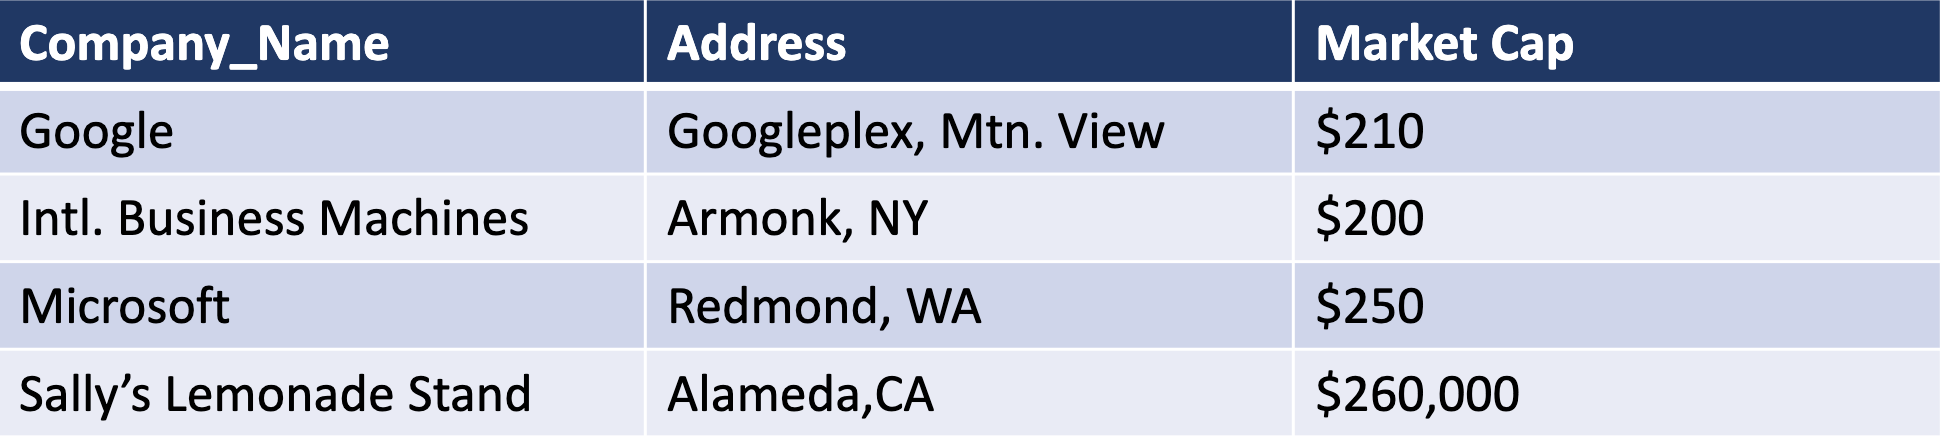
\includegraphics[width=\textwidth]{1.png}
\begin{itemize}
    \item Apple: Missing Data
    \item IBM: Entity Resolution / Unnormalized Naming
    \item Sally's Lemonade Stand: Unit Mismatch
\end{itemize}
\subsection{Where is Data Cleaning in the Organization?}
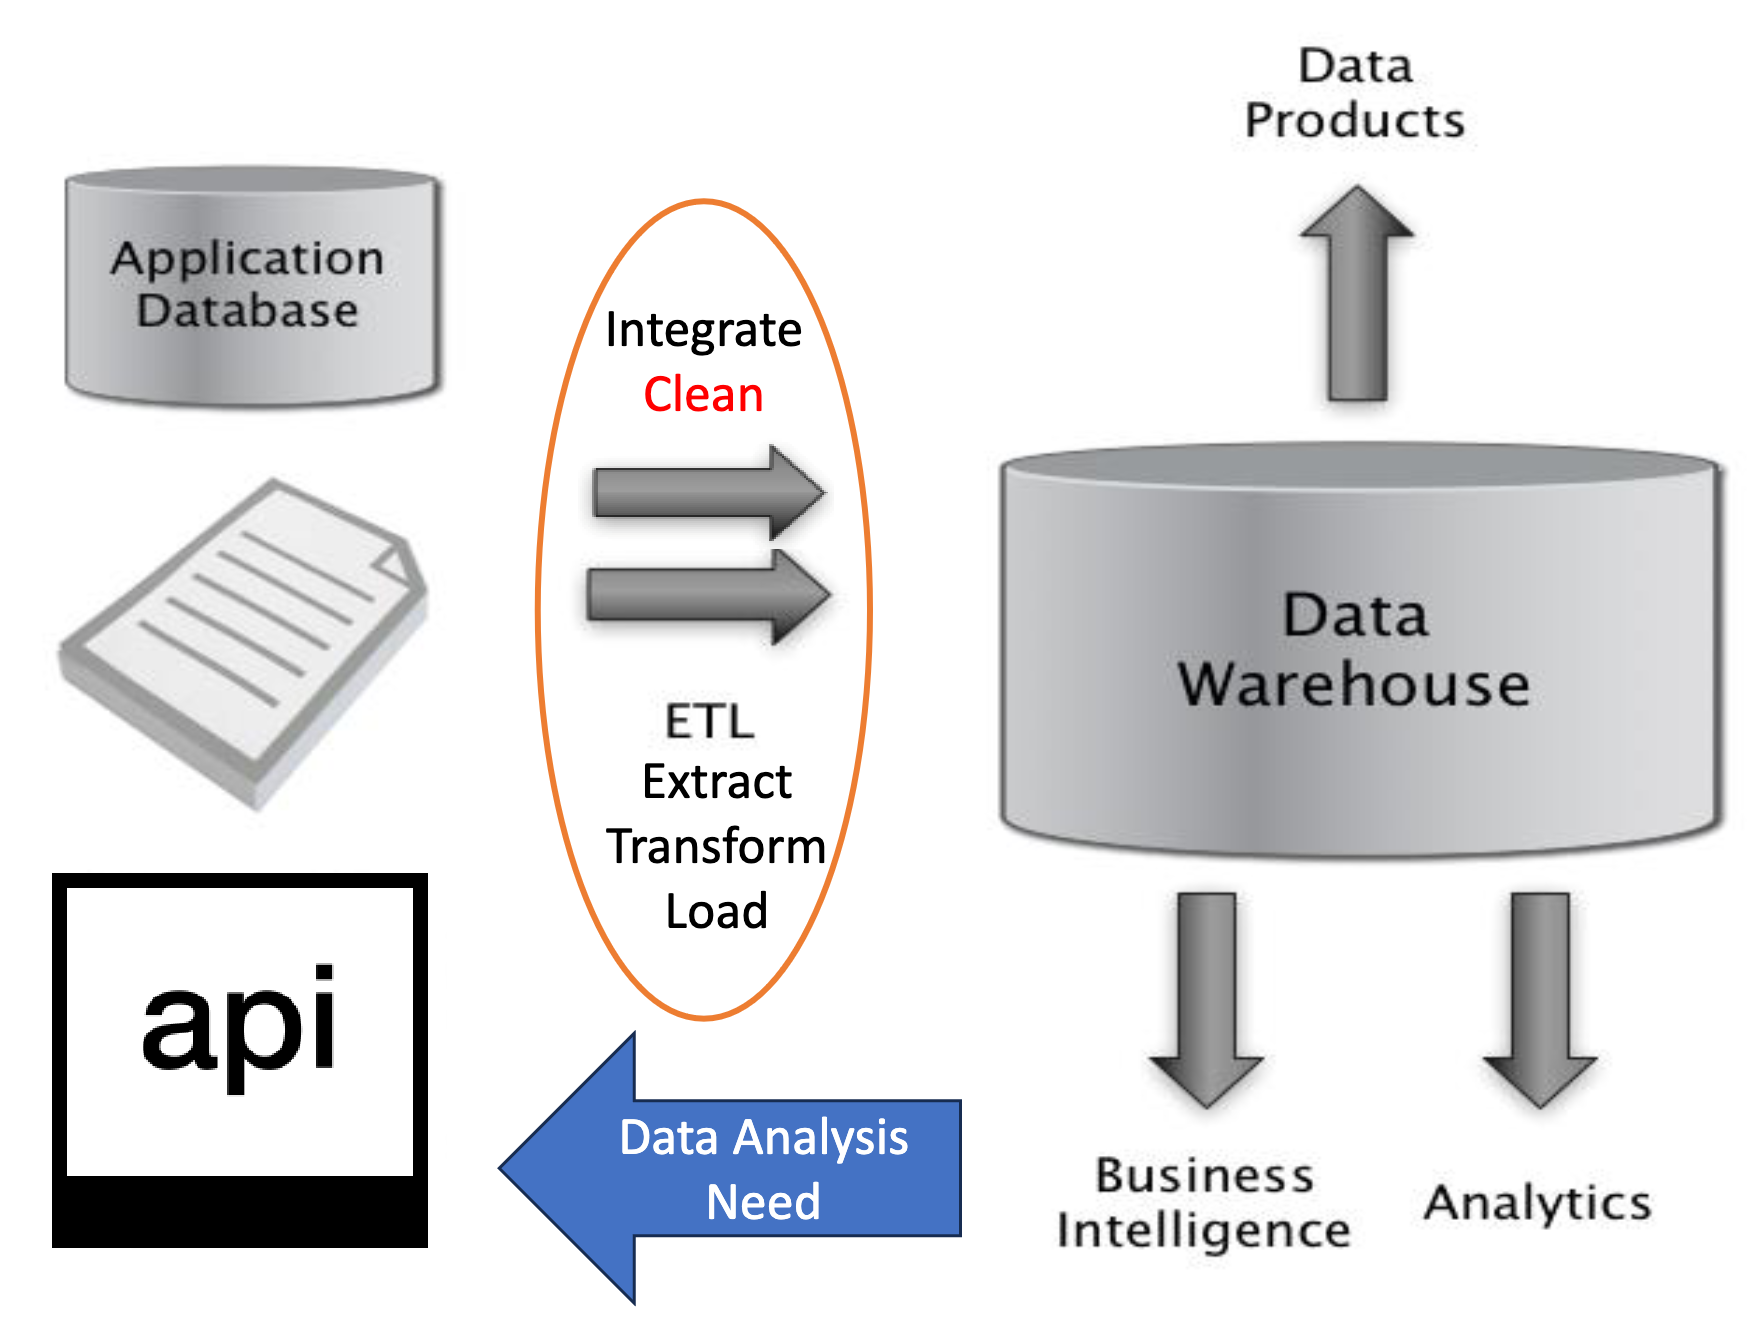
\includegraphics[width=\textwidth/2]{2.png}
\begin{itemize}
    \item Data comes in all shapres and forms
    \item ETL: Extract, Transform, Load
    \item Data science exists in business intelligence and analytics
    \item Data engineers work in application database
\end{itemize}
\subsection{Cost of Bad Quality Data Over Time}
\begin{itemize}
    \item Cost for preventing bad data: \$1
    \item Cost for correcting bad data: \$10
    \item Cost for fixing problem resulting from bad data: \$100
\end{itemize}

\section{Perspectives on Data Science
and Data Cleaning}
\subsection{Data Science is an Intersectional Discipline}
\begin{itemize}
    \item Computer Science
    \item Math and Statistics
    \item Domain Knowledge
\end{itemize}
\subsection{Dirty Data}
\begin{itemize}
    \item The Statistics View:
    \begin{itemize}
        \item There is a process that produces data
        \item Any dataset is a sample of the output of that process
        \item Results are probabilistic
        \item You can correct bias in your sample
    \end{itemize}
    \item The Database View:
    \begin{itemize}
        \item I got my hands on this data set
        \item Some of the values are missing, corrupted, wrong, duplicated
        \item Results are absolute (relational model)
        \item You get a better answer by improving the quality of the values in your dataset
    \end{itemize}
    \item The Domain Expert’s View
    \begin{itemize}
        \item This Data Doesn’t look right
        \item This Answer Doesn’t look right
        \item What happened?
    \end{itemize}
    \item The data scientist's view is a combination of the above.
\end{itemize}
\begin{note}
    A Data scientist knows more programming than a statistician
    and more statistics than a programmer.
    A Data scientist intimately understands their domain!
\end{note}
\subsection{Data Quality Problems}
\begin{itemize}
    \item Data is dirty on its own
    \begin{itemize}
        \item Human collection or data entry (generally lazy and want to see their children)
    \end{itemize}
    \item Data sets are clean but integration (i.e., combining them)
    screws them up (such as different units of measurement)
    \item Data sets are clean but suffer “bit rot” (lose data from cutting)
    \begin{itemize}
        \item Constant data transformations introduce errors, noise, data loss
        \item Meanings of labels change over time
    \end{itemize}
    \item Any combination of the above... and much, much more!
\end{itemize}
\subsection{Some Data Issues you will Encounter}
\begin{enumerate}
    \item Parsing text into fields (separator issues)
    \item Naming conventions and entity resolution D: NYC vs New York
    \item Missing required field (birthdate)
    \item Gaps in time series
    \item Different representations (“2” vs 2), Unicode lookalikes
    \item Fields too long (get truncated)
    \item Mixed data types (feet, meters)
    \item Redundant Records (exact match or other)
    \item Formatting issues – especially dates
    \item Licensing issues/privacy/cost prevent access to all data
\end{enumerate}
\subsection{Key Types of Data Quality Issues}
\begin{itemize}
    \item \textbf{incomplete}: lacking attribute values, lacking certain attributes
    of interest, or containing only aggregate data
    \begin{itemize}
        \item e.g., occupation=“ ”
    \end{itemize}
    \item \textbf{noisy}: containing errors or outliers
    \begin{itemize}
        \item e.g., Salary=“-10”
    \end{itemize}
    \item \textbf{inconsistent}: containing discrepancies in codes or names
    \begin{itemize}
        \item e.g., Age=“42” Birthday=“03/07/1997”
        \item e.g., Was rating “1,2,3”, now rating “A, B, C”
        \item e.g., discrepancy between duplicate records
    \end{itemize}
    \item \textbf{redundancy}: duplicated content
\end{itemize}
\subsection{Why Is Data Dirty?}
\begin{itemize}
    \item Incomplete data may come from
    \begin{itemize}
        \item “Not applicable” data value when collected
        \item Changes in the data collected over time
        \item Human/hardware/software problems
    \end{itemize}
    \item Noisy data (incorrect values) may come from
    \begin{itemize}
        \item Faulty data collection instruments, undocumented API changes
        \item Human or computer error at data entry, UI changes!
        \item Errors in data transmission, discretization, conversion (losing precision)
        \item Typing errors (meters, feet, km mixed in same column)
    \end{itemize}
    \item Inconsistent data may come from
    \begin{itemize}
        \item Different data sources (data integration)
        \item Changes in data collection practices over time
    \end{itemize}
    \item Redundancy
    \begin{itemize}
        \item Human error (could not find previous record), data integration
    \end{itemize}
\end{itemize}
\section{The Role of Data Cleaning in
Data Science}
\subsection{Data Science in the Real World}
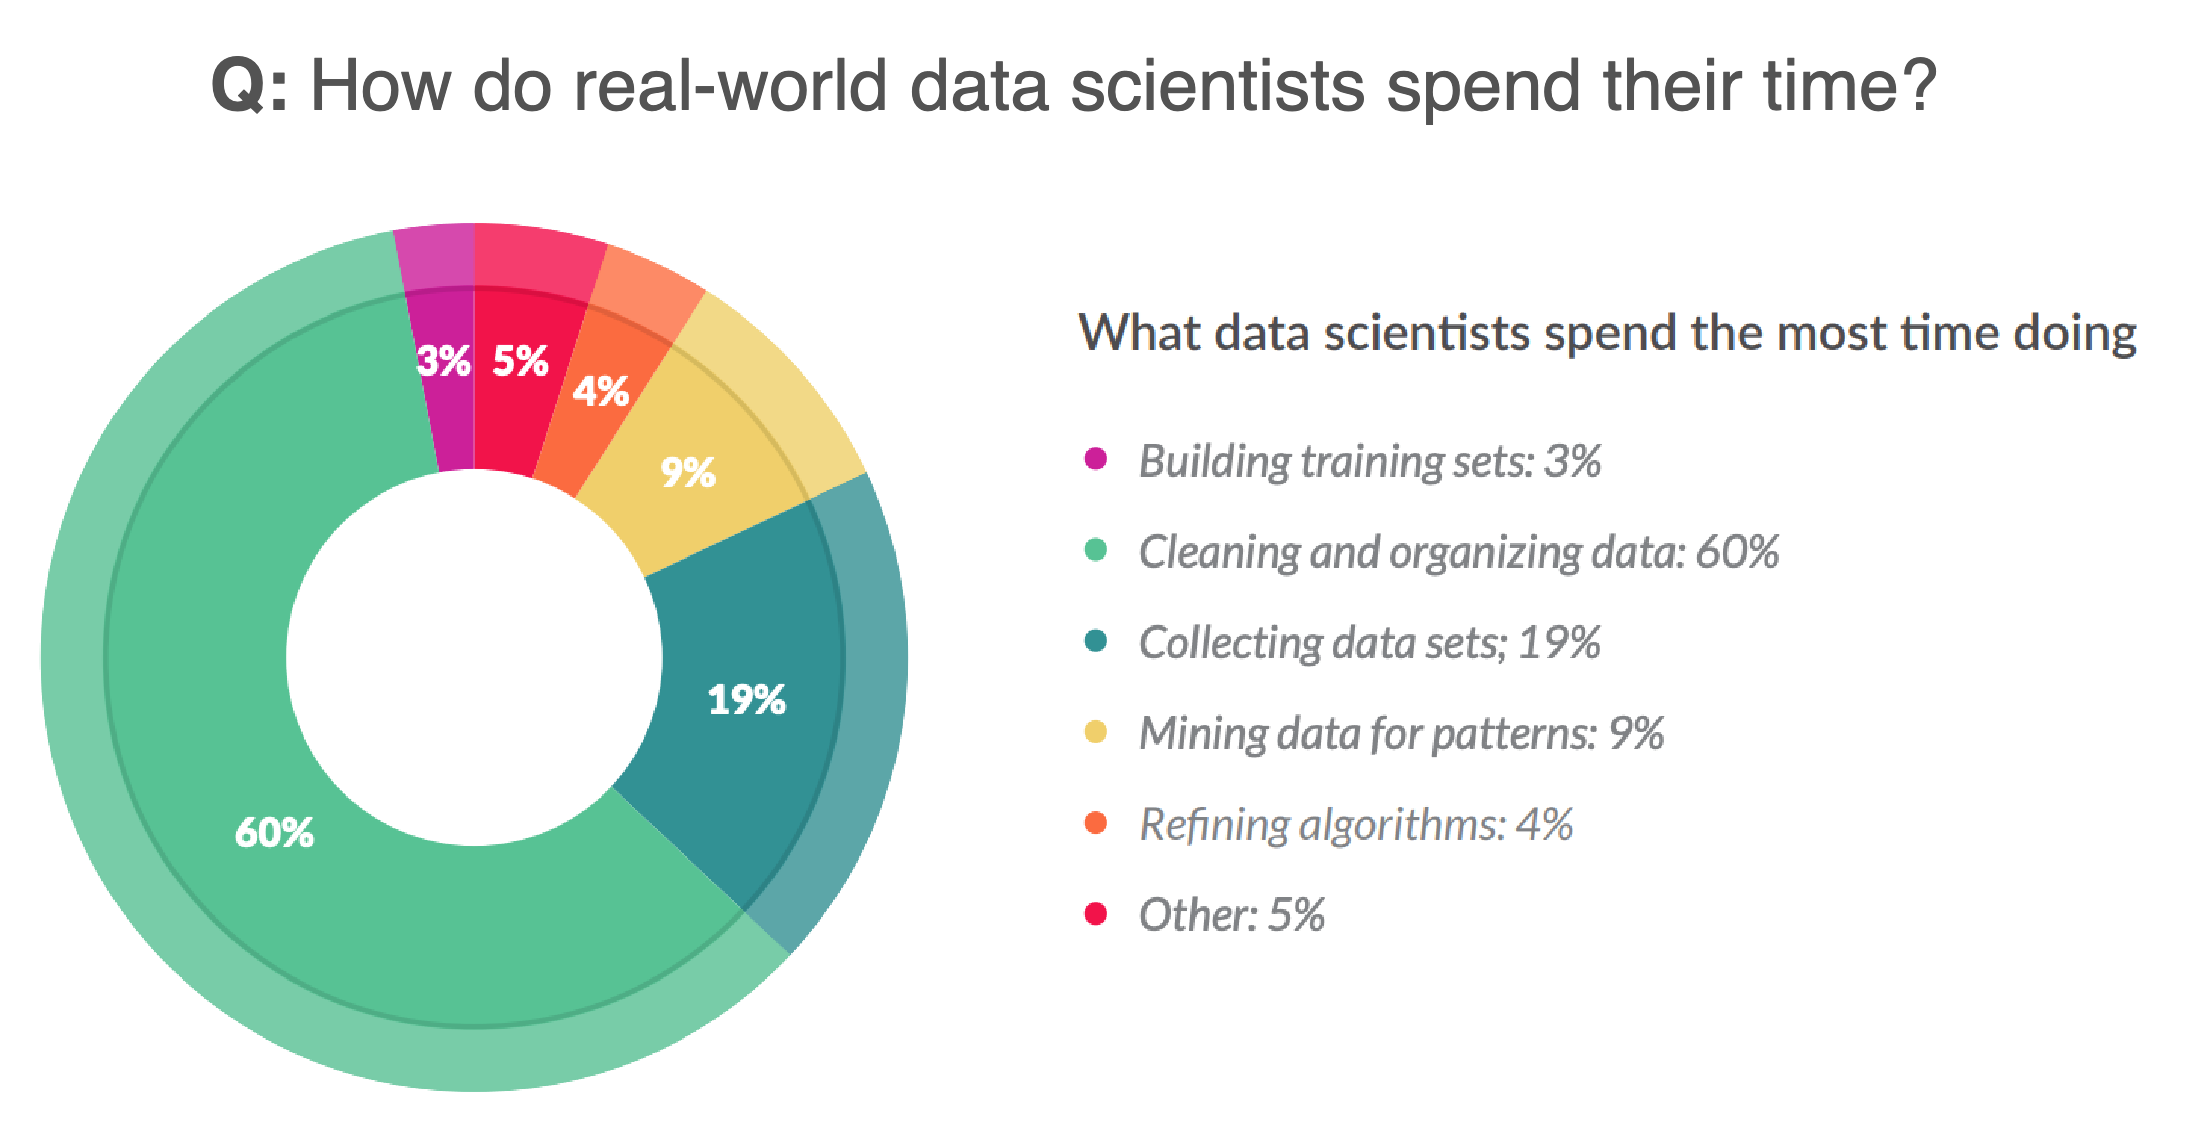
\includegraphics[width=\textwidth]{3.png}


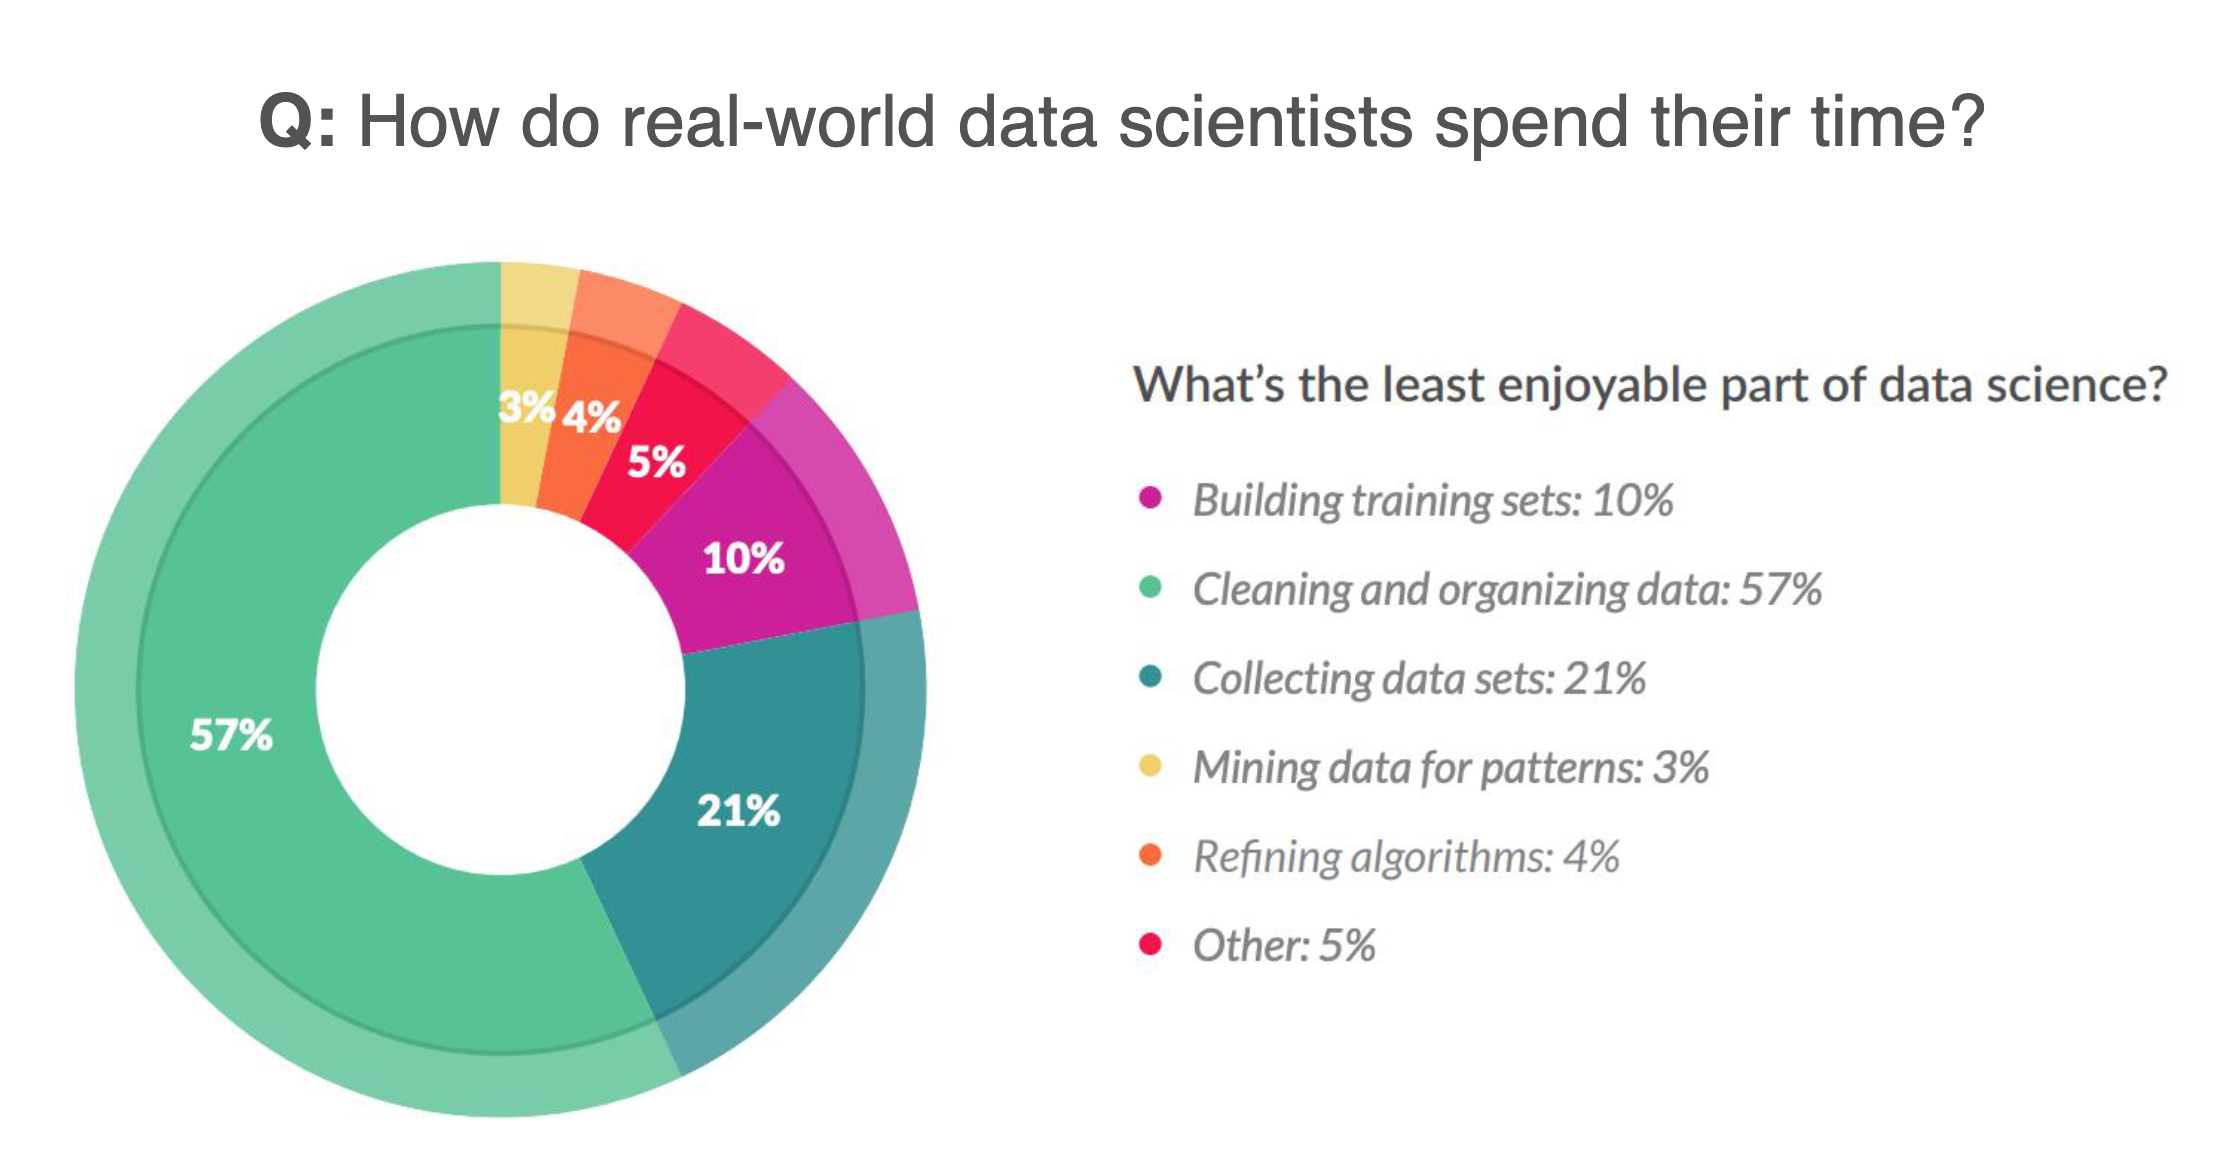
\includegraphics[width=\textwidth]{4.png}
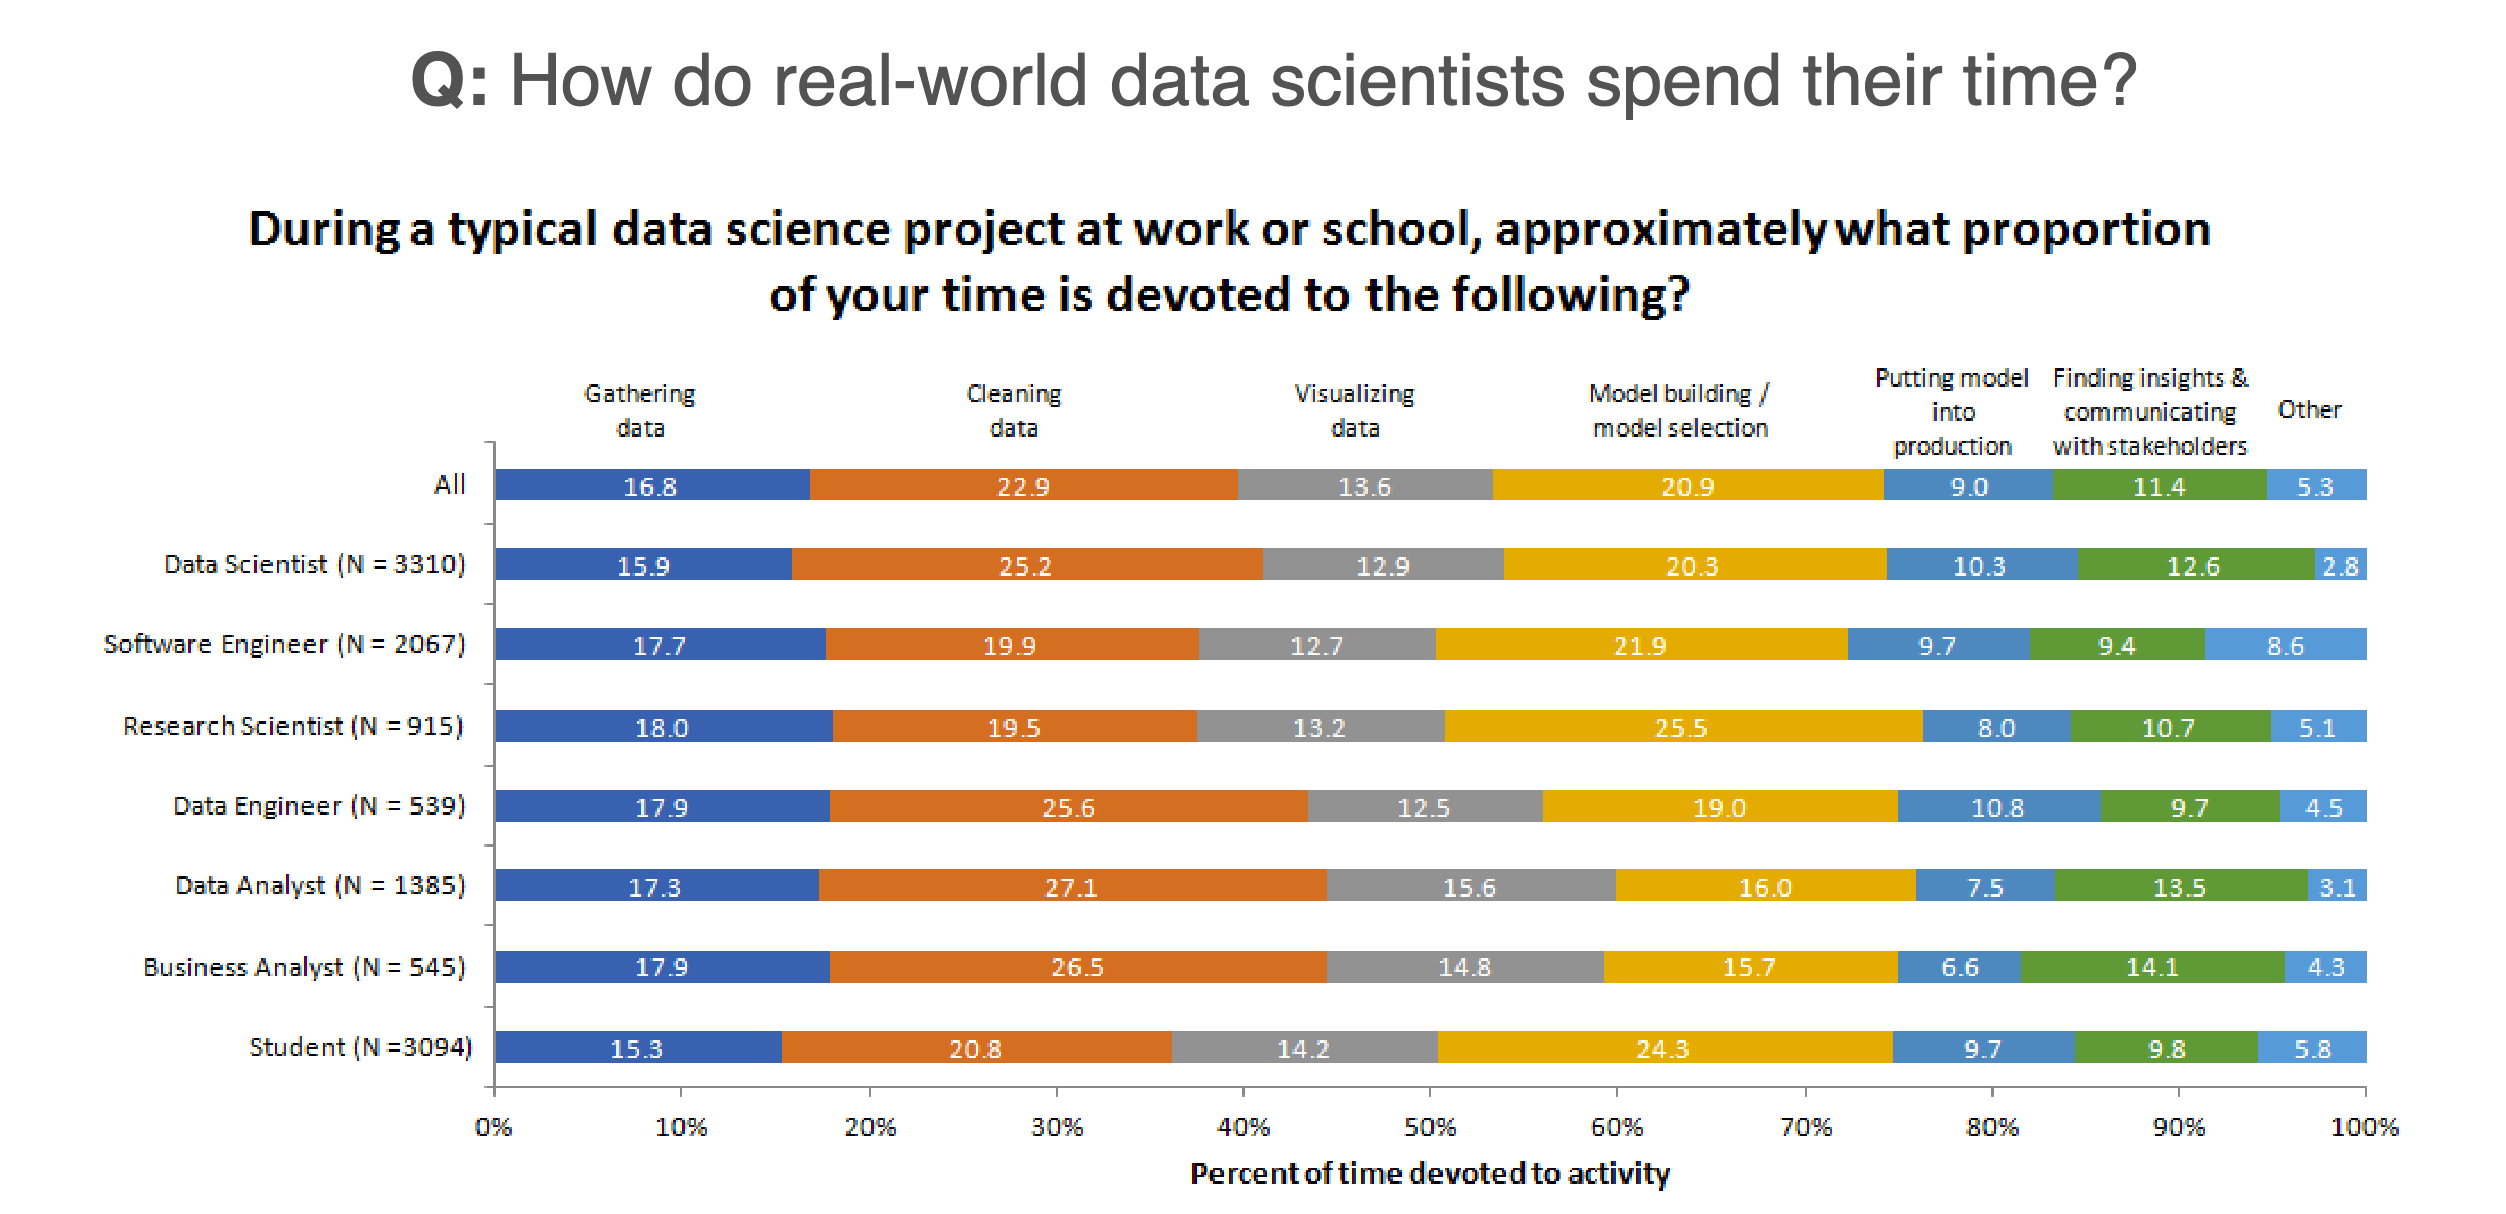
\includegraphics[width=\textwidth]{5.png}
\subsection{Data Cleaning Makes Everything Okay?}
\begin{note}
    “The appearance of a hole in the
earth's ozone layer over
Antarctica, first detected in 1976,
was so unexpected that scientists
didn't pay attention to what their
instruments were telling them;
they thought their instruments
were malfunctioning.”
- National Center for
Atmospheric Research
\end{note}
The data was rejected as unreasonable by data quality control algorithms.
% 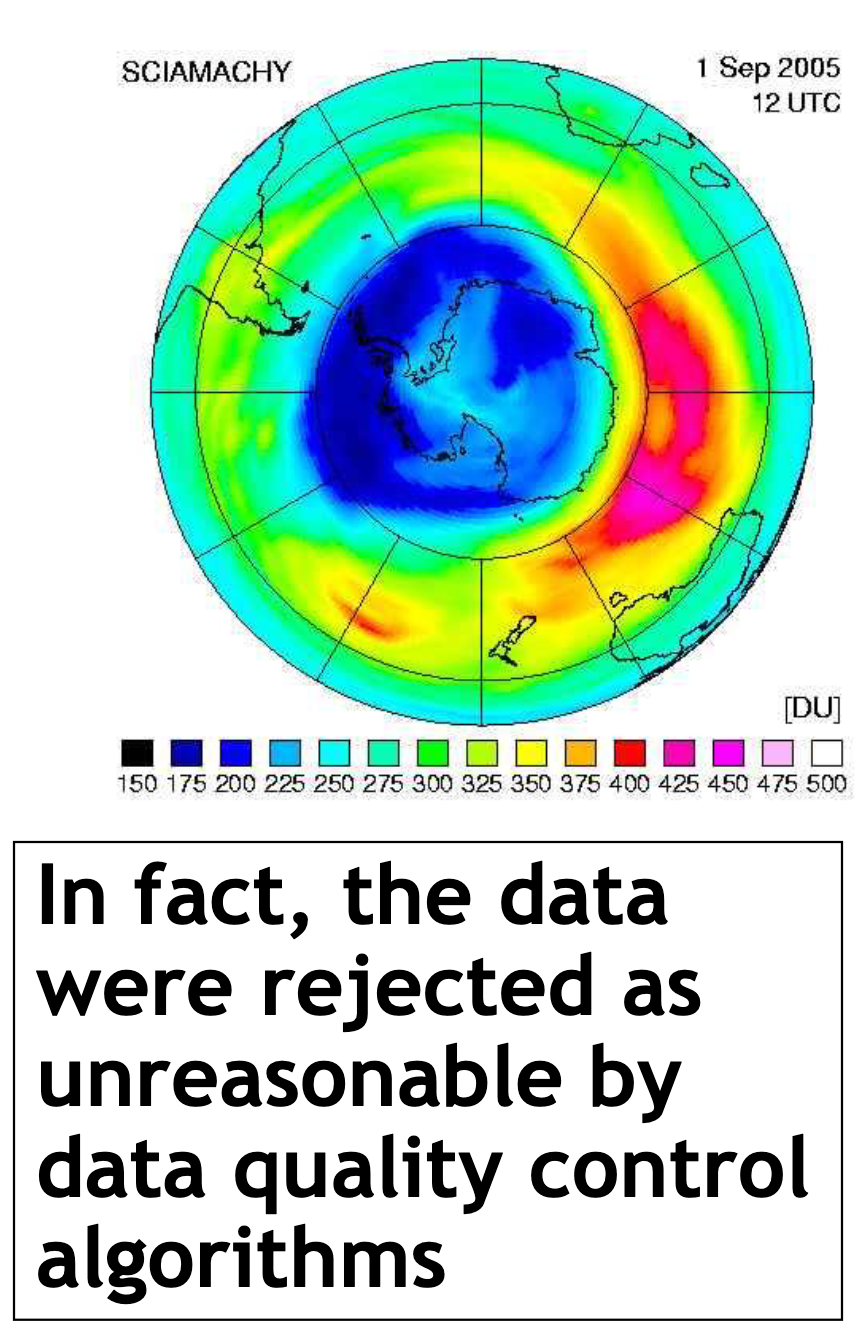
\includegraphics[width=\textwidth/3]{6.png}
\section{Principles of Data Cleaning}
\subsection{Data Cleaning Tasks}
\begin{itemize}
    \item Data Summary
    \item Consider filling in missing values
    \item Identify outliers and smooth out noisy data
    \item Correct inconsistent data
    \item Resolve redundancy
\end{itemize}
\section{Data Cleaning: Data Summary}
\subsection{Data Summary Procedure}
\begin{itemize}
    \item Look at data types of columns
    \begin{itemize}
        \item Beware of "Object" columns, indicator that you've mixed types (e.g., "2" and 2)
    \end{itemize}
    \item For high cardinality strings and categorical (e.g,. "country") columns
    \begin{itemize}
        \item How many unique elements are there?
        \item Are any missing?
        \item Count frequencies of string
        \begin{itemize}
            \item Look at top-10 most frequent and least frequent values
            \item Look at strings near the mean and median frequency
        \end{itemize}
    \end{itemize}
    \item For low cardinality strings and categorical (e.g,. “province") columns
    \begin{itemize}
        \item Look at frequency of each unique value
    \end{itemize}
    \item For ordinal numeric (integers) or floating point values
    \begin{itemize}
        \item Compute summary statistics
        \item View a histogram (but before you do this, hypothesize what you will see)
    \end{itemize}
\end{itemize}
\subsection{Summary Statistics and for Each Variable (Column)}
\begin{itemize}
    \item Range
    \begin{itemize}
        \item Minimum
        \item Maximum
    \end{itemize}
    \item Central Tendency
    \begin{itemize}
        \item Mean
        \item Median
        \item Mode
        \begin{itemize}
            \item Value that occurs most frequently in discrete data
            \item Value with highest frequency (or value range with highest frequency) in continuous data
            \item Informally: \# peaks in numeric data – unimodal, bimodal, trimodal, multimodal, ...
        \end{itemize}
    \end{itemize}
    \item If Data is non-numeric, consider frequencies below (e.g., mean frequency of jobs in “Job”)
    \item If Data is a string, consider sorting it and looking at nearby values
\end{itemize}
\subsection{Measuring the Dispersion of Data}
\begin{itemize}
    \item Quartiles, outliers and boxplots
    \begin{itemize}
        \item Quartiles: Q1 (25th percentile), Q3 (75th percentile)
        \item Inter-quartile range: IQR = Q3 – Q1
        \item Five number summary: min, Q1, M, Q3, max
        \item Boxplot: ends of the box are the quartiles, median is marked, whiskers (min / max),
        and plot outlier individually
        \item Outlier: usually, a value higher/lower than 1.5 x IQR
    \end{itemize}
    \item Variance and standard deviation (sample: s, population: $\sigma$)
    \begin{itemize}
        \item Variance: (algebraic, scalable computation)
        \item 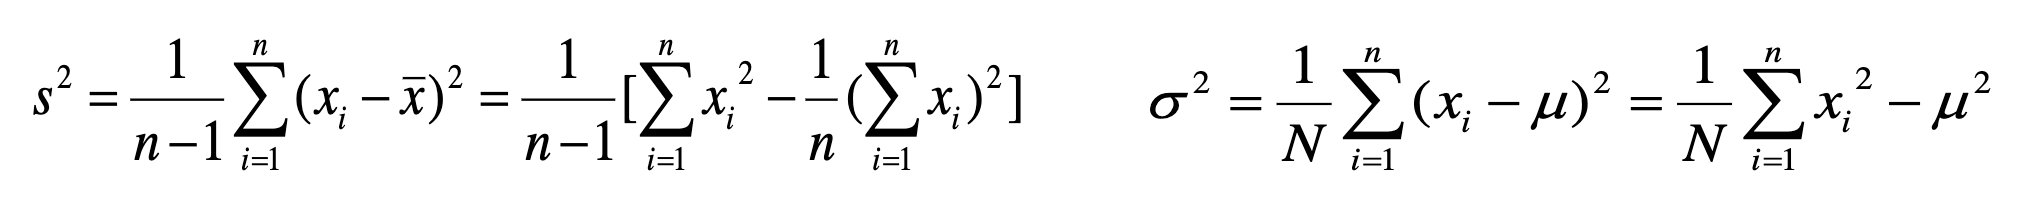
\includegraphics[width=\textwidth - 51.46509pt]{7.png}
        \item Standard deviation $s$ (or $\sigma$) is the square root of variance $s^2$ (or $\sigma^2$)
    \end{itemize}
\end{itemize}
\subsection{Boxplot Analysis}
\begin{itemize}
    \item Five-number summary of a distribution:
    \begin{itemize}
        \item Minimum, Q1, M, Q3, Maximum (IQR=Q3-Q1)
    \end{itemize}
    \item Historical Boxplot
    \begin{itemize}
        \item Data is represented with a box
        \item The ends of the box are at the first and third
        quartiles (Q1,Q3), i.e., the height of the box is IQR
        \item The median is marked by a line within the box
        \item Whiskers: two lines outside the box extend to
        Minimum and Maximum
        \item Shows asymmetry unlike mean ± std 
    \end{itemize}
\end{itemize}
\begin{note}
    Beware boxplots can hide multimodality.
    
    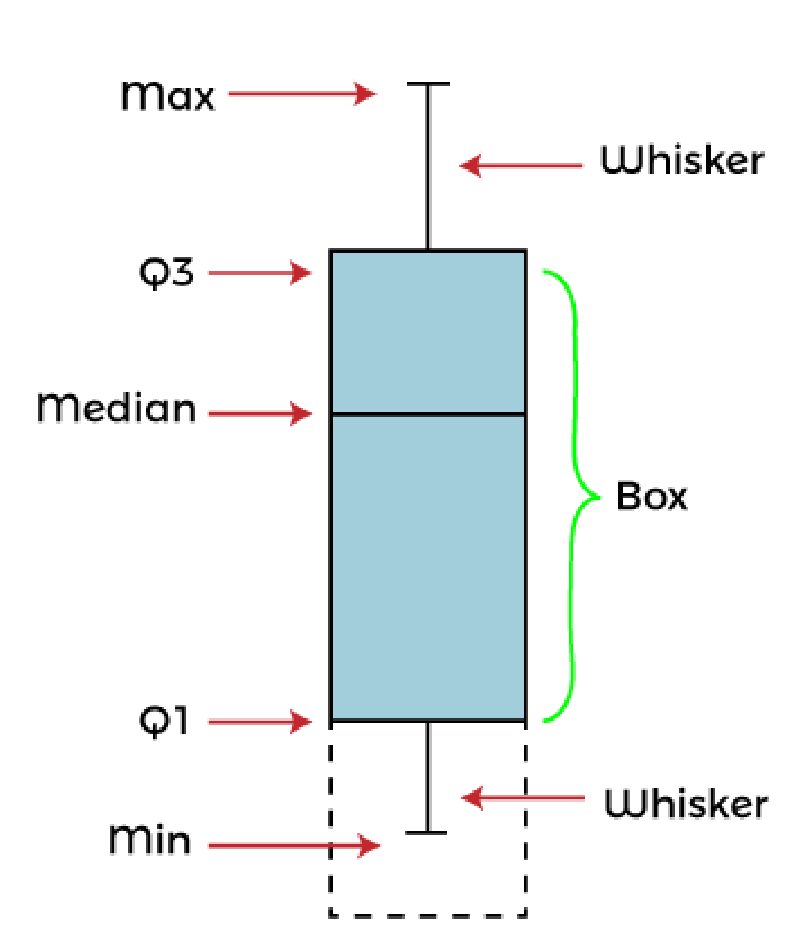
\includegraphics[height=\textheight/4]{8.png}
\end{note}
\subsection{Python Boxplot (not all Boxplots are the same)}
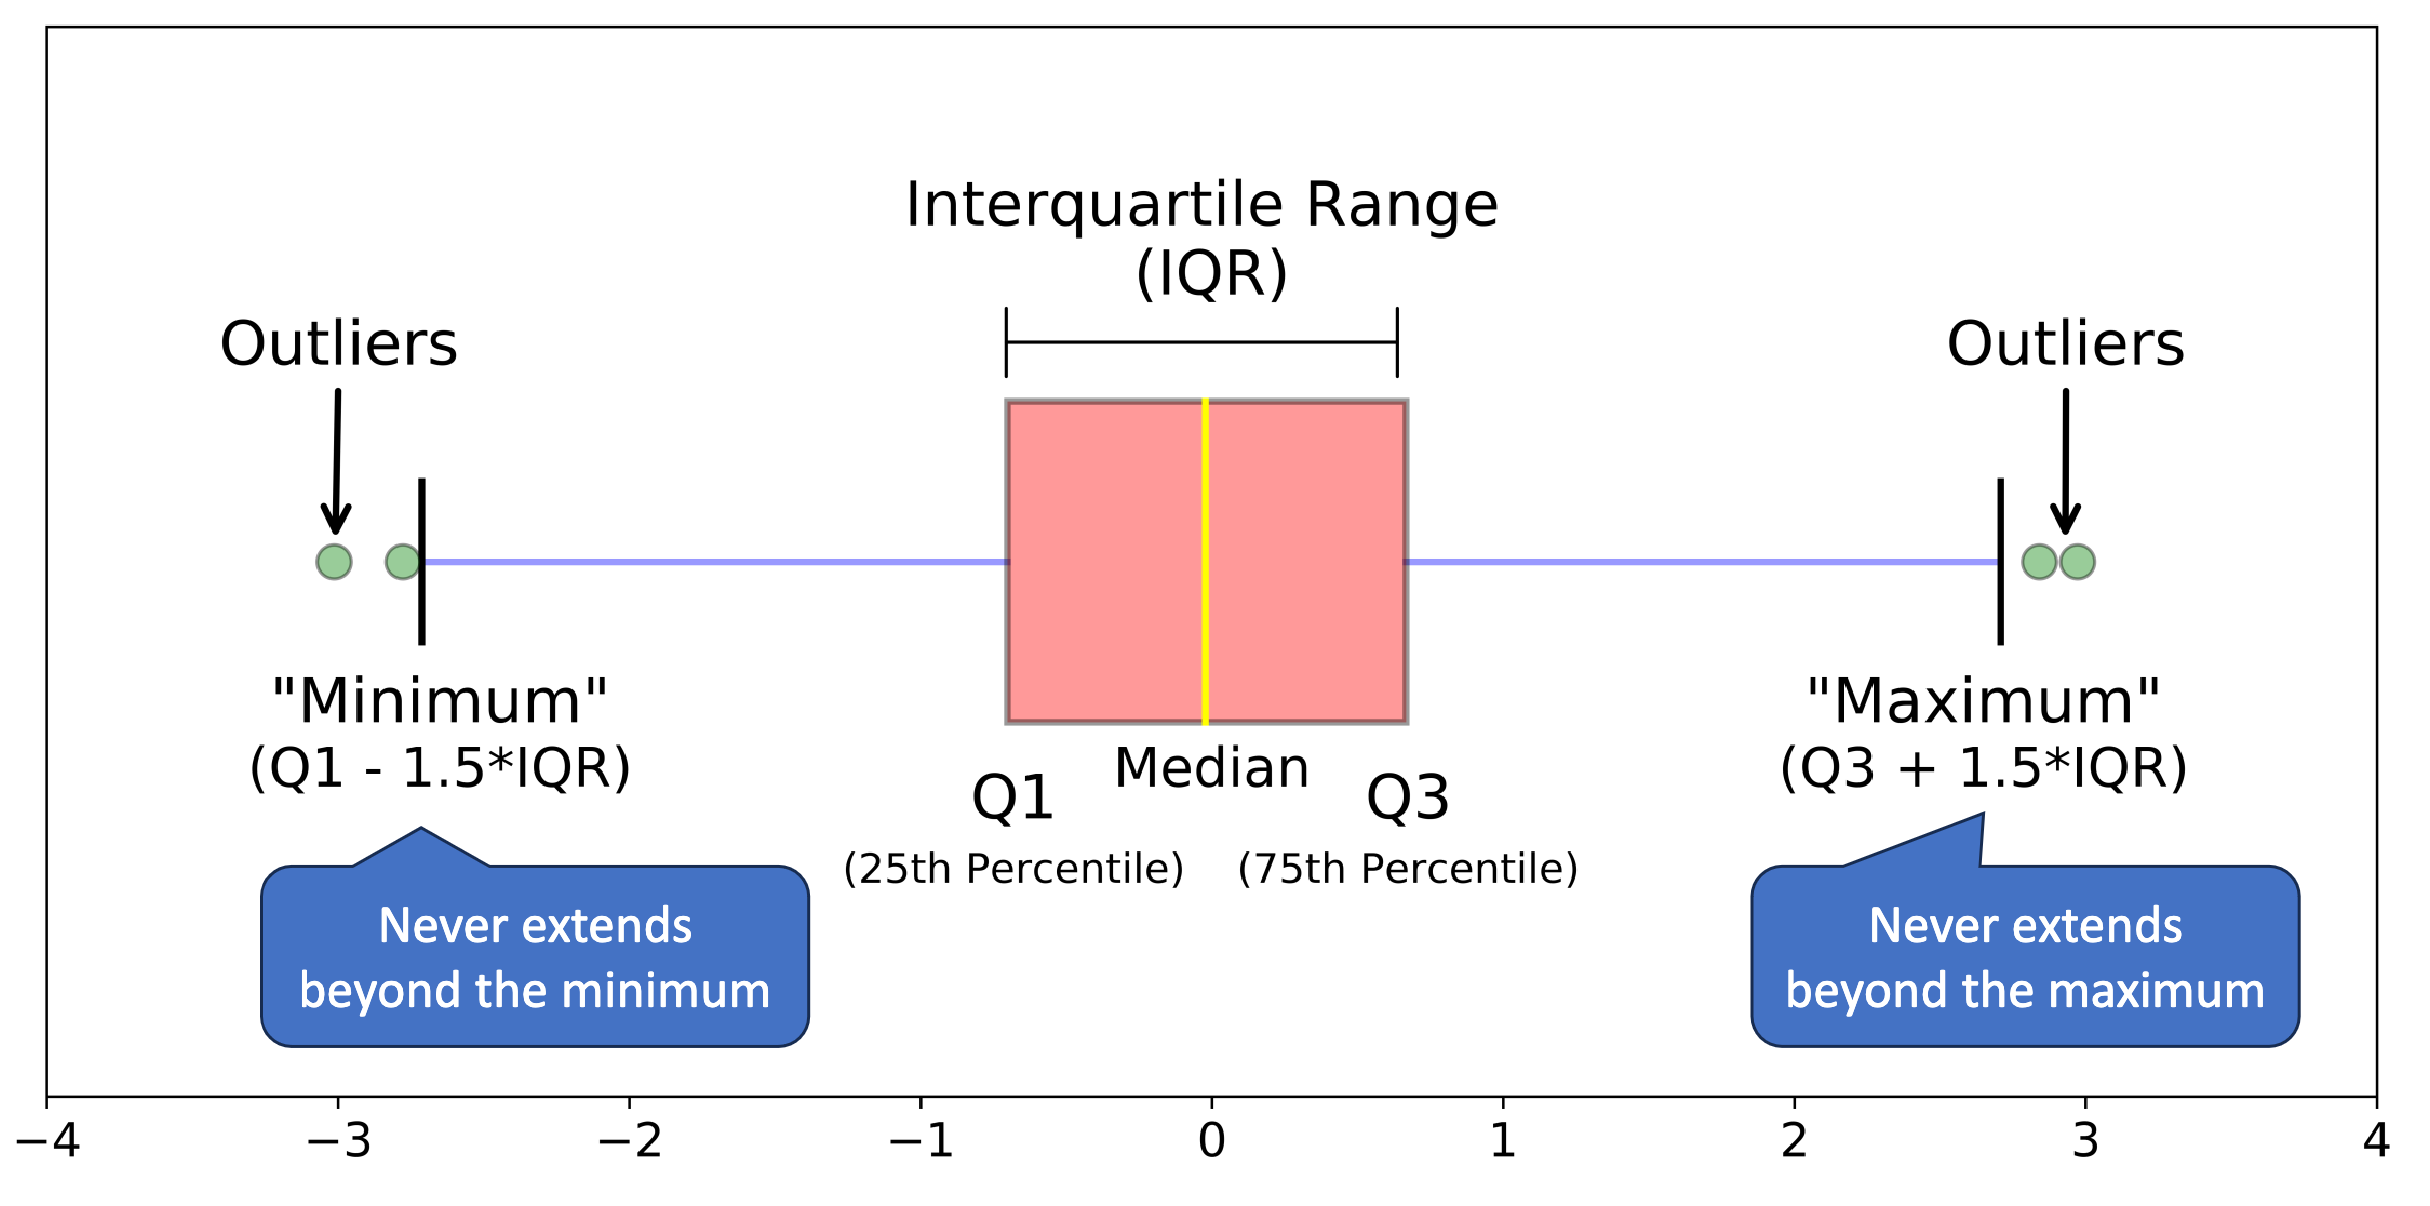
\includegraphics[width=\textwidth]{9.png}
\subsection{Understanding the Data Distribution: Histograms}
\begin{note}
    The normal distribution is unimodal.
\end{note}
\begin{itemize}
    \item Summary statistics
    like standard deviation
    can be very misleading if
    you don’t know the
    distribution
    \item A Histogram shows an
    empirical density
    \begin{itemize}
        \item I.e., the frequency of
        binned value ranges of
        your variable (column)
        \item Use a bar chart of
        frequencies if variable is
        discrete
    \end{itemize}
\end{itemize}
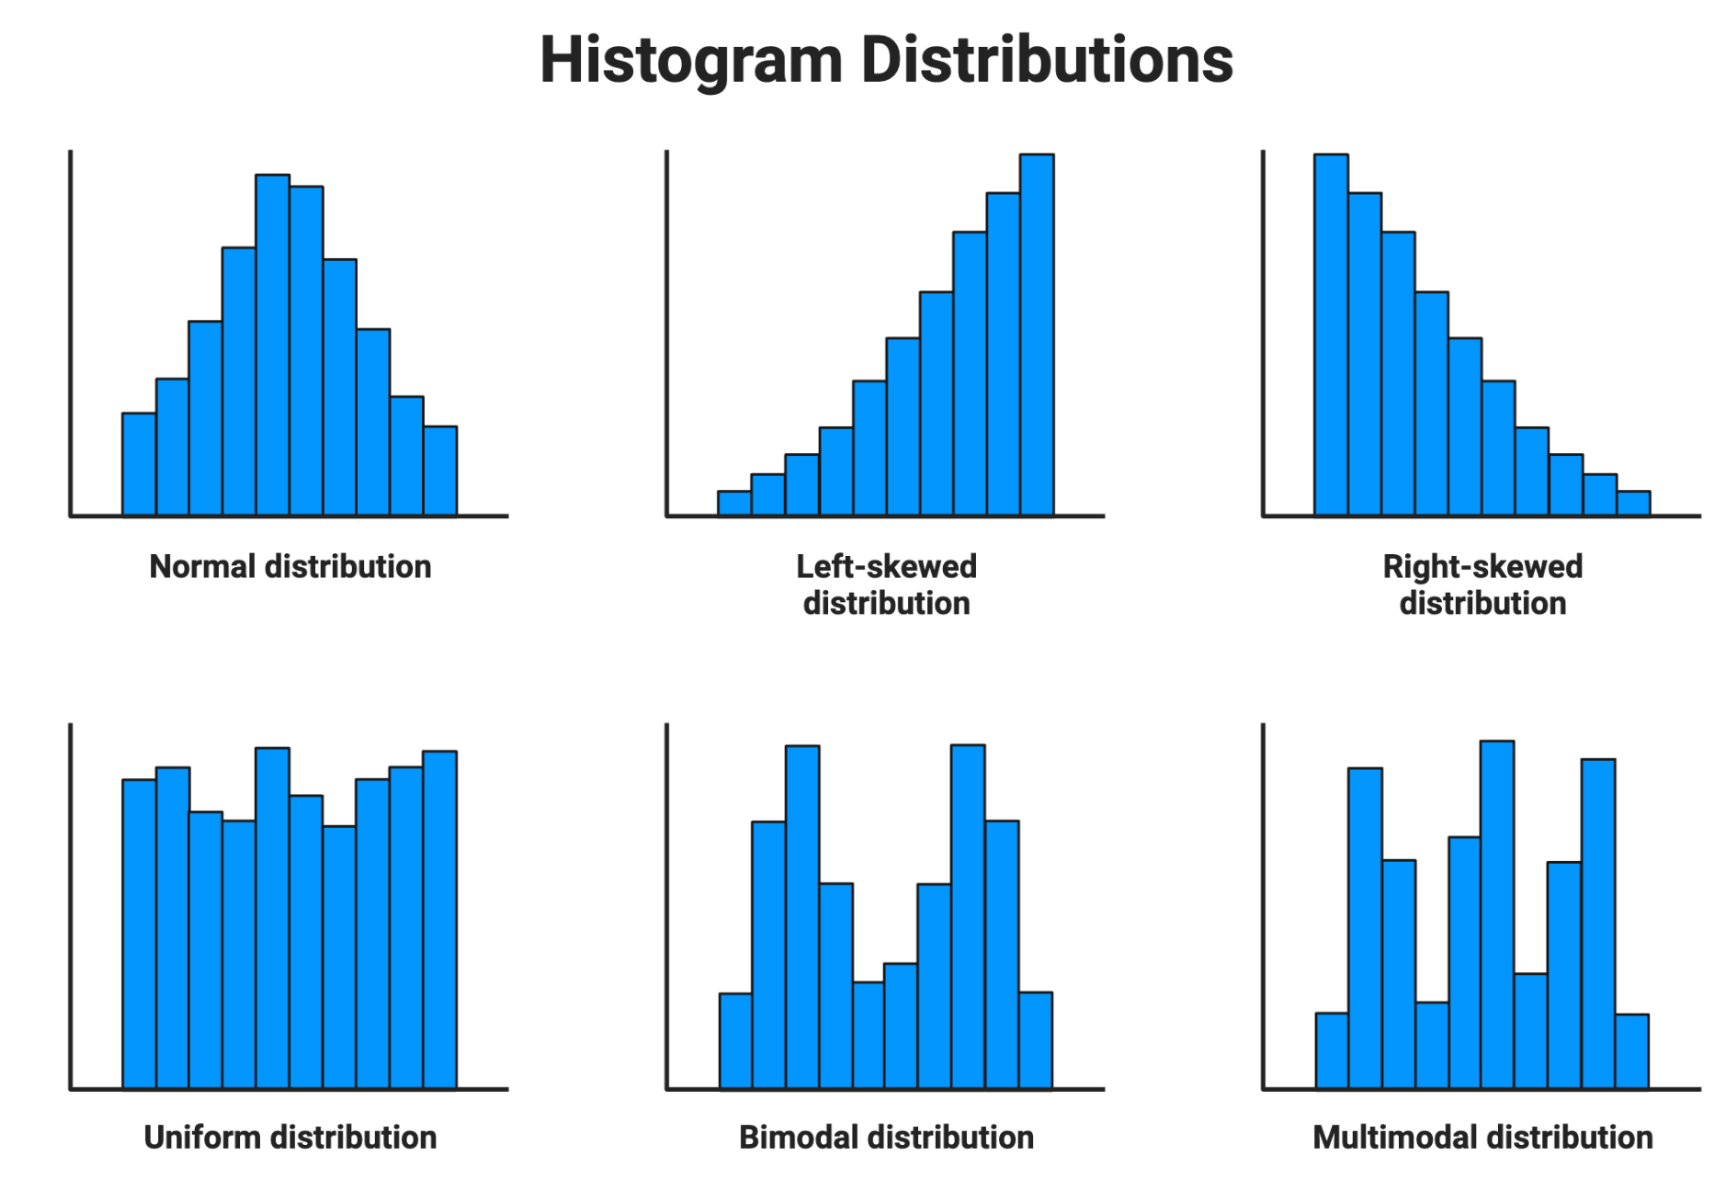
\includegraphics[width=\textwidth]{10.png}
\subsection{Processes Generate Different Distributions}
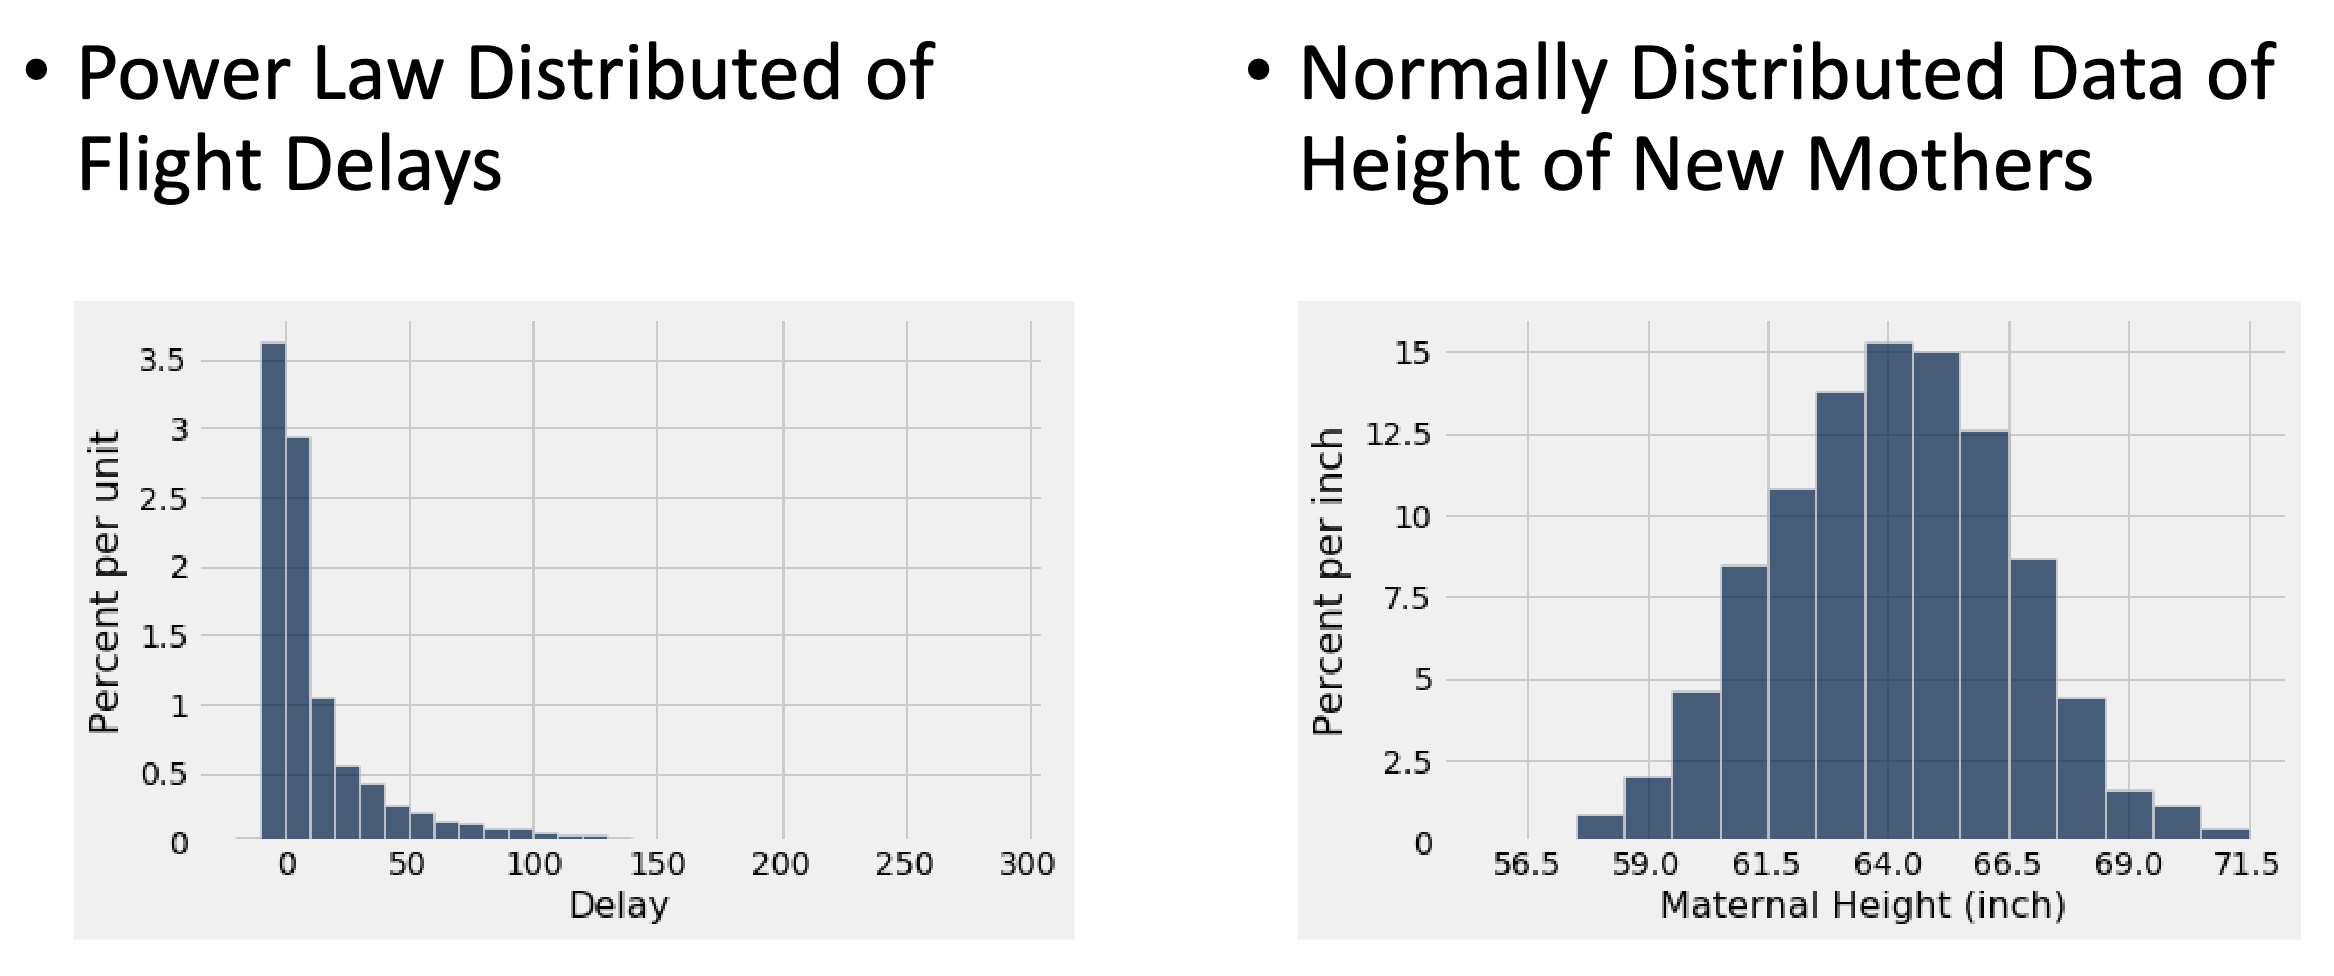
\includegraphics[width=\textwidth]{11.png}
\begin{itemize}
    \item Mean, median, and mode are same for Gaussian data, but (very) different for power law data.
\end{itemize}
\subsection{Symmetric vs. Skewed Data}
\begin{itemize}
    \item Median, mean and mode of symmetric,
    positively and negatively skewed data
\end{itemize}
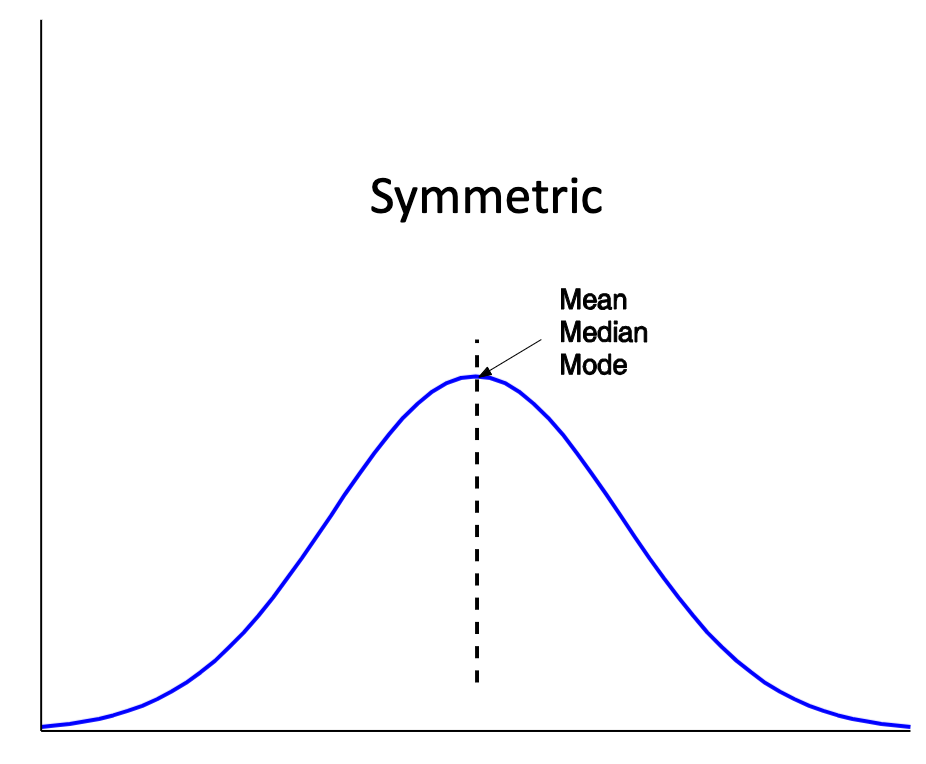
\includegraphics[width=\textwidth/4]{12.png}
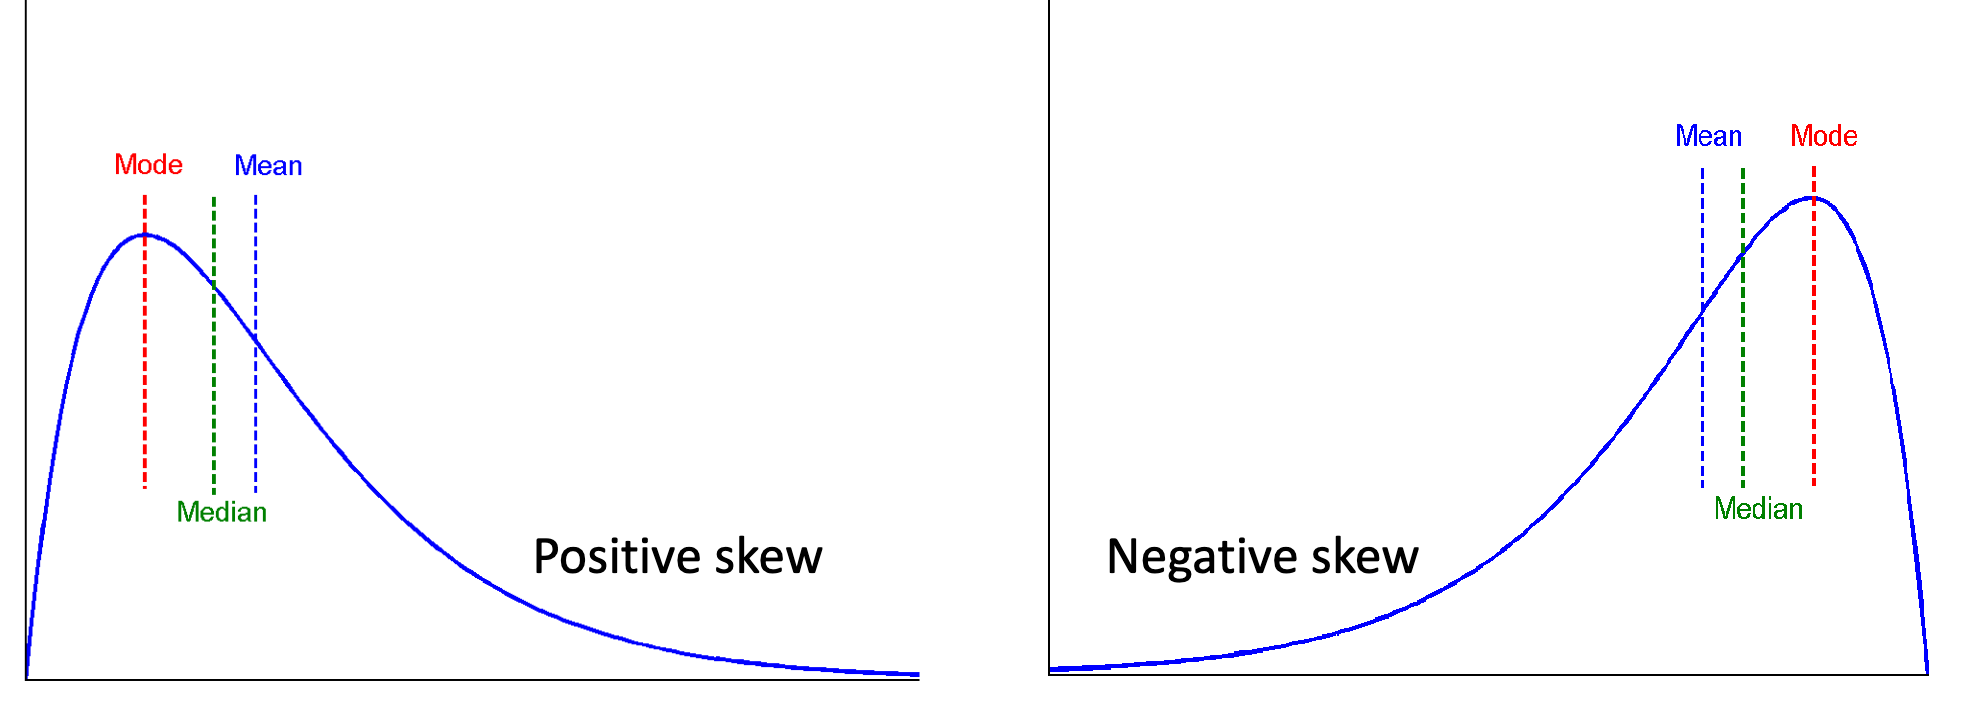
\includegraphics[width=\textwidth]{13.png}
\subsection{Properties of Normal Distribution Curve}
\begin{itemize}
    \item The normal (distribution) curve
    \item From $\mu$–$\sigma$ to $\mu$+$\sigma$: contains about 68\% of the measurements
    ($\mu$: mean, $\sigma$: standard deviation)
    \item From $\mu$–2$\sigma$ to $\mu$+2$\sigma$: contains about 95\% of it
    \item From $\mu$–3$\sigma$ to $\mu$+3$\sigma$: contains about 99.7\% of it
    \item Useful for interpreting z-scores (cf. transformation slides)
\end{itemize}
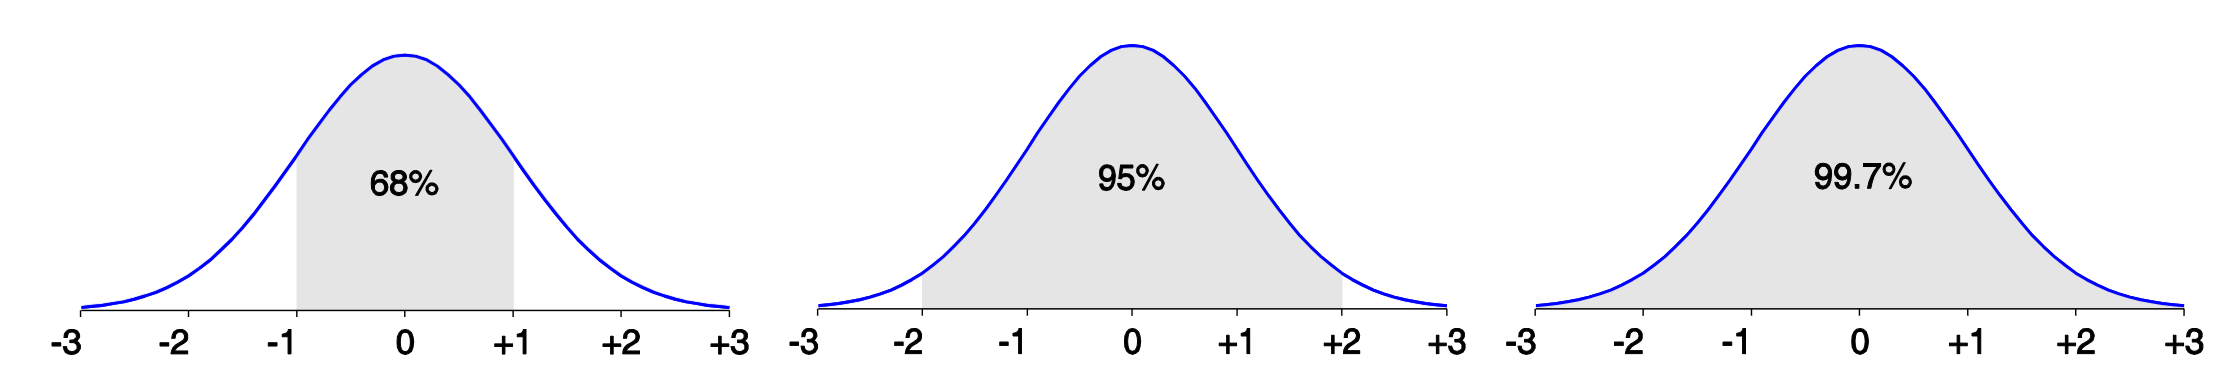
\includegraphics[width=\textwidth]{14.png}
\section{Data Cleaning: Missing Values}
\subsection{Missing Values}
\begin{note}
    It's important to understand how your data is missing.
\end{note}
\begin{itemize}
    \item Missing Completely at Random (MCAR): the random process by which data is
    missing does not depend on any other observed (i.e., column) nor latent
    (i.e., unobserved) variable
    \begin{itemize}
        \item e.g., for column "income" uniformly randomly pick a row and with probability P, delete the
        "income" entry at that row
    \end{itemize}
    \item Missing at Random (MAR): the random process by which the data is missing
    depends on another variable (column), but not on a latent (unobserved) variable
    \begin{itemize}
        \item e.g., for column "income" uniformly randomly pick a row and with probability P if that row has
        "gender=Male" or probability Q if that row has "gender=Female", delete "income" at that row
        \item \textbf{it can depend on the row itself, but not on the missing value}
    \end{itemize}
    \item Missing Not at Random (MNAR): the random process by which the data is missing depends on a latent variable
    \begin{itemize}
        \item e.g., for column "income" delete the "income" at a row *if* the day the row is added to the
        table is on a Monday (where the timestamp of when a row was added is not recorded in any
        column and is hence latent)
        \item e.g., for column "income", the "income" at a row is missing if it was below \$10,000 – here, the
        value that made it missing is not recorded in the table and therefore a latent cause
    \end{itemize}
\end{itemize}
\subsection{Example Customer Data}
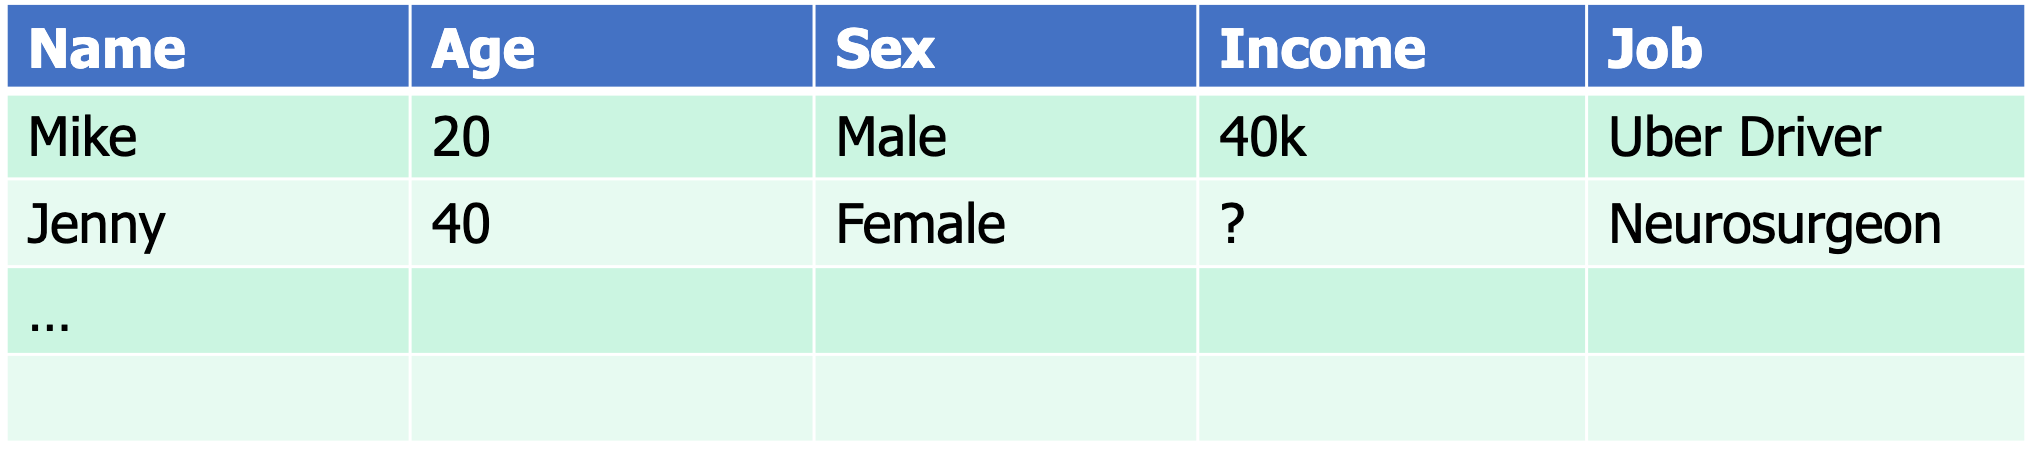
\includegraphics[width=\textwidth]{15.png}
\subsection{Imputation}
\begin{itemize}
    \item Imputation is risky (makes assumptions and “creates” missing values)
    \begin{itemize}
        \item If very few rows are missing data, it may be better to delete those rows
        \item But if high rate of missingness, cannot delete most of data!
    \end{itemize}
    \item Some downstream analysis requires complete data in rows
    \begin{itemize}
        \item Correlation between all pairs of variables
        \item Classification and regression in most of machine / deep learning
    \end{itemize}
    \item Impute if you must, but imputer beware
    \begin{itemize}
        \item As they said in Ancient Rome: caveat imputor
    \end{itemize}
\end{itemize}
\subsection{Imputation Methods}
\begin{itemize}
    \item String or categorical data
    \begin{itemize}
        \item Most frequent value (or mode)
    \end{itemize}
    \item Integer data
    \begin{itemize}
        \item Median makes more sense than mean (because it is an integer value)
        \item Mode? (consider conditional mode)
    \end{itemize}
    \item Continuous (floating point) data
    \begin{itemize}
        \item Mean
        \item Median (can differ significantly from Mean for asymmetric distribution)
    \end{itemize}
    \item Consider a specific value if MNAR
    \begin{itemize}
        \item No response to a survey could mean “No” be default
    \end{itemize}
\end{itemize}
\subsection{Conditional Imputation}
\begin{itemize}
    \item But wait, we can also conditionally impute!
    \begin{itemize}
        \item Can use “groupby” and aggregation on one or more other columns
        \begin{itemize}
            \item E.g., Impute “Income” conditioned on median income grouped by “Job”
        \end{itemize}
        \item Could train a classifier or predictor from other columns (be careful)
    \end{itemize}
    \item If Data is MCAR
    \begin{itemize}
        \item Consider how other columns may impact prediction
        \begin{itemize}
            \item E.g., “Sex=male” gives a strong hint about “Is Pregnant?”
        \end{itemize}
    \end{itemize}
    \item If Data is MAR
    \begin{itemize}
        \item Consider if the missingness condition should influence the prediction
        \begin{itemize}
            \item E.g., all stores in “North Yorkville” did not report client income
        \end{itemize}
        \item Note: columns that influence missingness do not necessarily influence the prediction
        \begin{itemize}
            \item E.g., “Income” missing for “Location=Scarborough” but may be most influenced by “Age” and “Job”
        \end{itemize}
    \end{itemize}
\end{itemize}
\section{Data Cleaning: Noise,
Inconsistency, Redundancy}
\subsection{Reality Check from Summary Statistics and Domain Knowledge}
\begin{itemize}
    \item Range
    \begin{itemize}
        \item Minimum: height shouldn't be negative
        \item Maximum: can height be 3m? can be found in stats instead
    \end{itemize}
    \item Central Tendency:
    \begin{itemize}
        \item Mean: can mean height be 1.8m? (may be skewed by some outliers)
        \item Median: can median height be 1.8m? (says that half of the people are >= 1.8m)
        \item Mode: can mode height be 1.8m?
        \begin{itemize}
            \item Can height be multimodal? yes
        \end{itemize}
    \end{itemize}
    \item If Data is non-numeric, consider frequencies or percentages
    \begin{itemize}
        \item Can the most frequent word be “computer”?
        \item Can 75\% of the jobs in your database be neurosurgeon?
    \end{itemize}
    \item For sorted strings, do both “Microsft” and “Microsoft” appear?
\end{itemize}
\subsection{Identify Outliers and Potential Errors}
Could be bad values, poor data collection
\begin{note}
    Outliers can be real data, but they can also be errors. Your analysis is skewed by outliers if they are not truly outliers.
    They can be removed if they are not representative of the population you intend to analyze.
\end{note}


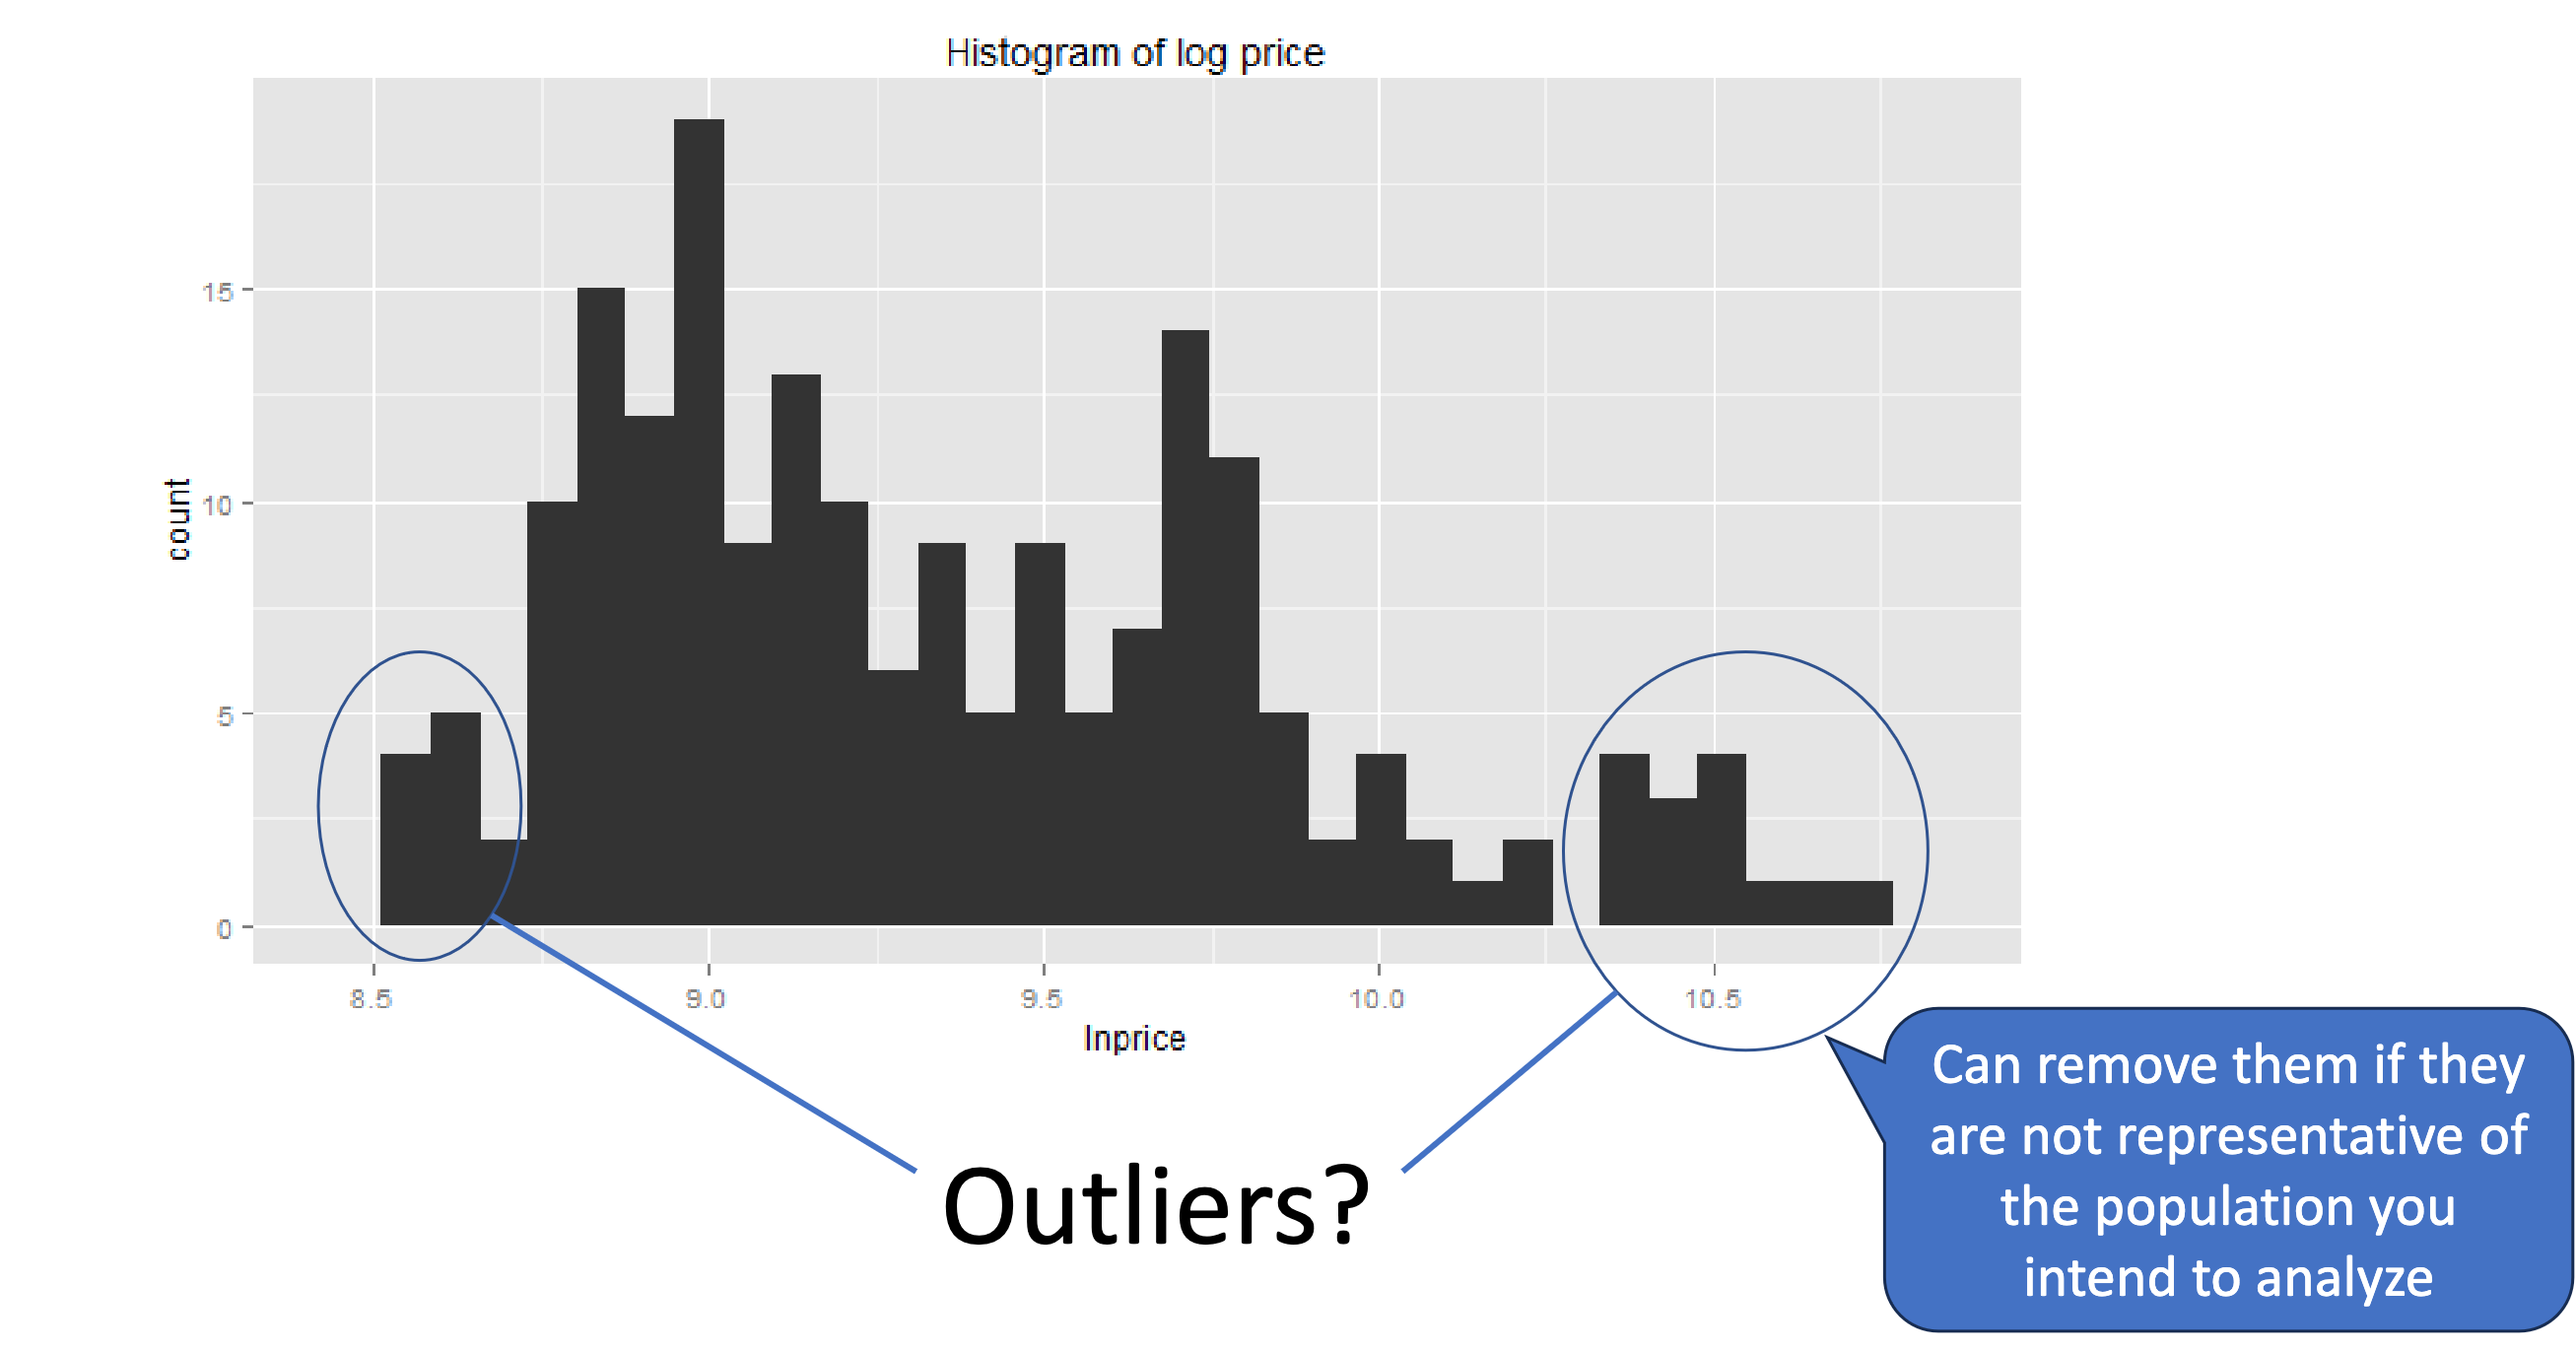
\includegraphics[width=\textwidth]{16.png}
\subsection{Data Cleaning Task: Entity Matching}
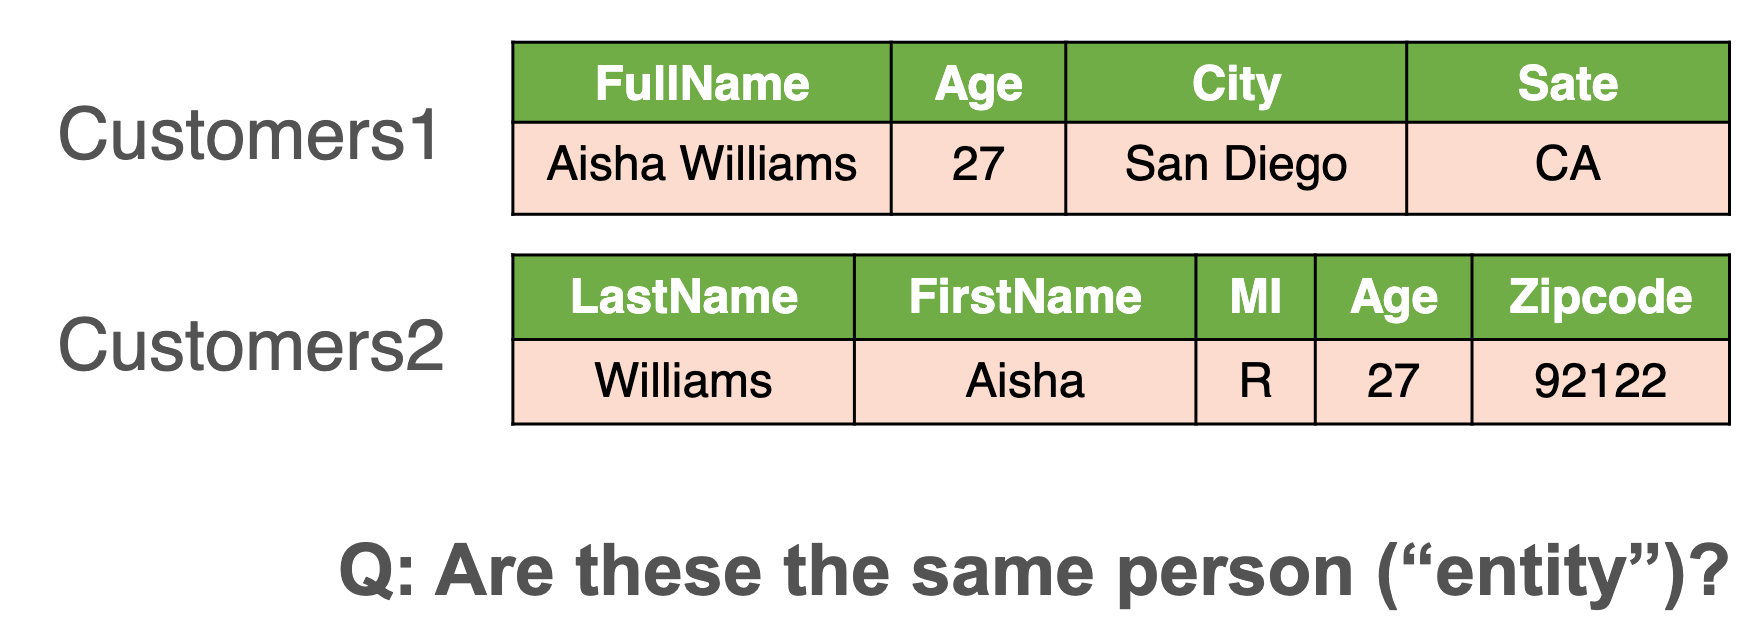
\includegraphics[width=\textwidth]{17.png}
\begin{itemize}
    \item Duplicates often occur in data integrated from multiple sources
    \item Or duplicates can simply result from redundant data entry
    \item Without merging / deduplication: will overcount records
    \begin{itemize}
        \item Deduplication methods provided by record linkage or entity linkage
    \end{itemize}
\end{itemize}
\newpage
\section{Data Transformation:
Improve Interpretability}
\subsection{Data Transformation}
\begin{itemize}
    \item Smoothing: remove noise from data by taking a local average
    \item Aggregation: summarization but lose the details
    \item Generalization: back off labels to a concept hierarchy
    \item Attribute/feature construction
    \begin{itemize}
        \item New attributes derived from the given ones
    \end{itemize}
    \item Normalization: scaled to fall within a small, specified range
    \begin{itemize}
        \item min-max normalization
        \item subtract mean (preserves magnitude)
        \item z-score normalization
        \item log normalization
    \end{itemize}
\end{itemize}
\subsection{Data Transformation: Normalization}
\begin{note}
    Min-Max normalization does not consider standard deviation. If your data is dynamic then the range changes, so Z-score is preferred as it is more stable.
\end{note}
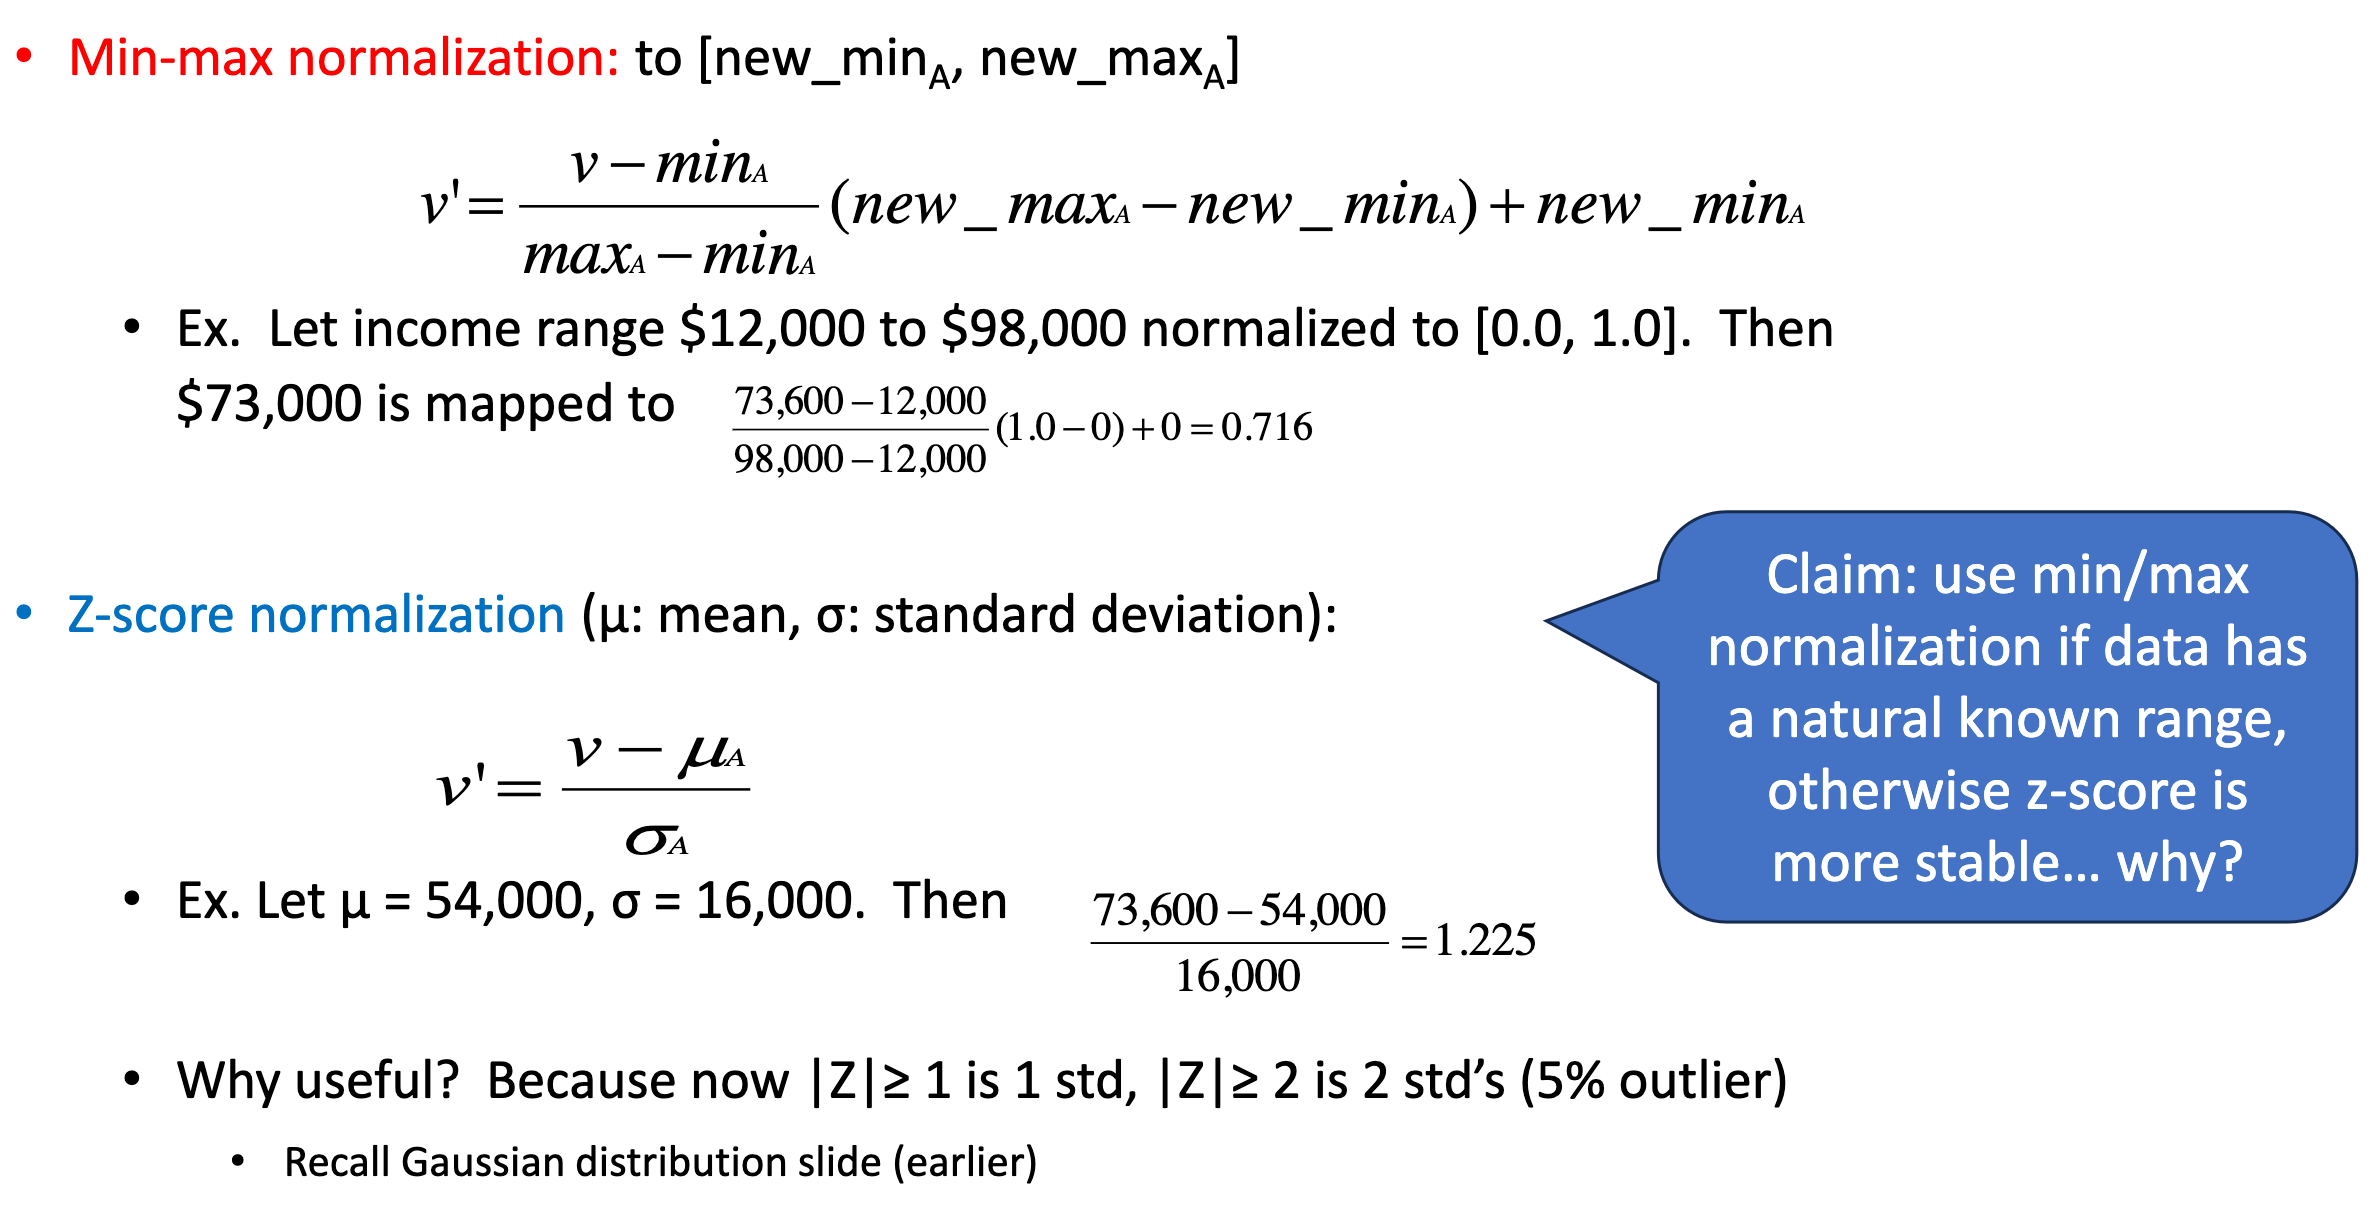
\includegraphics[width=\textwidth/2]{18.png}
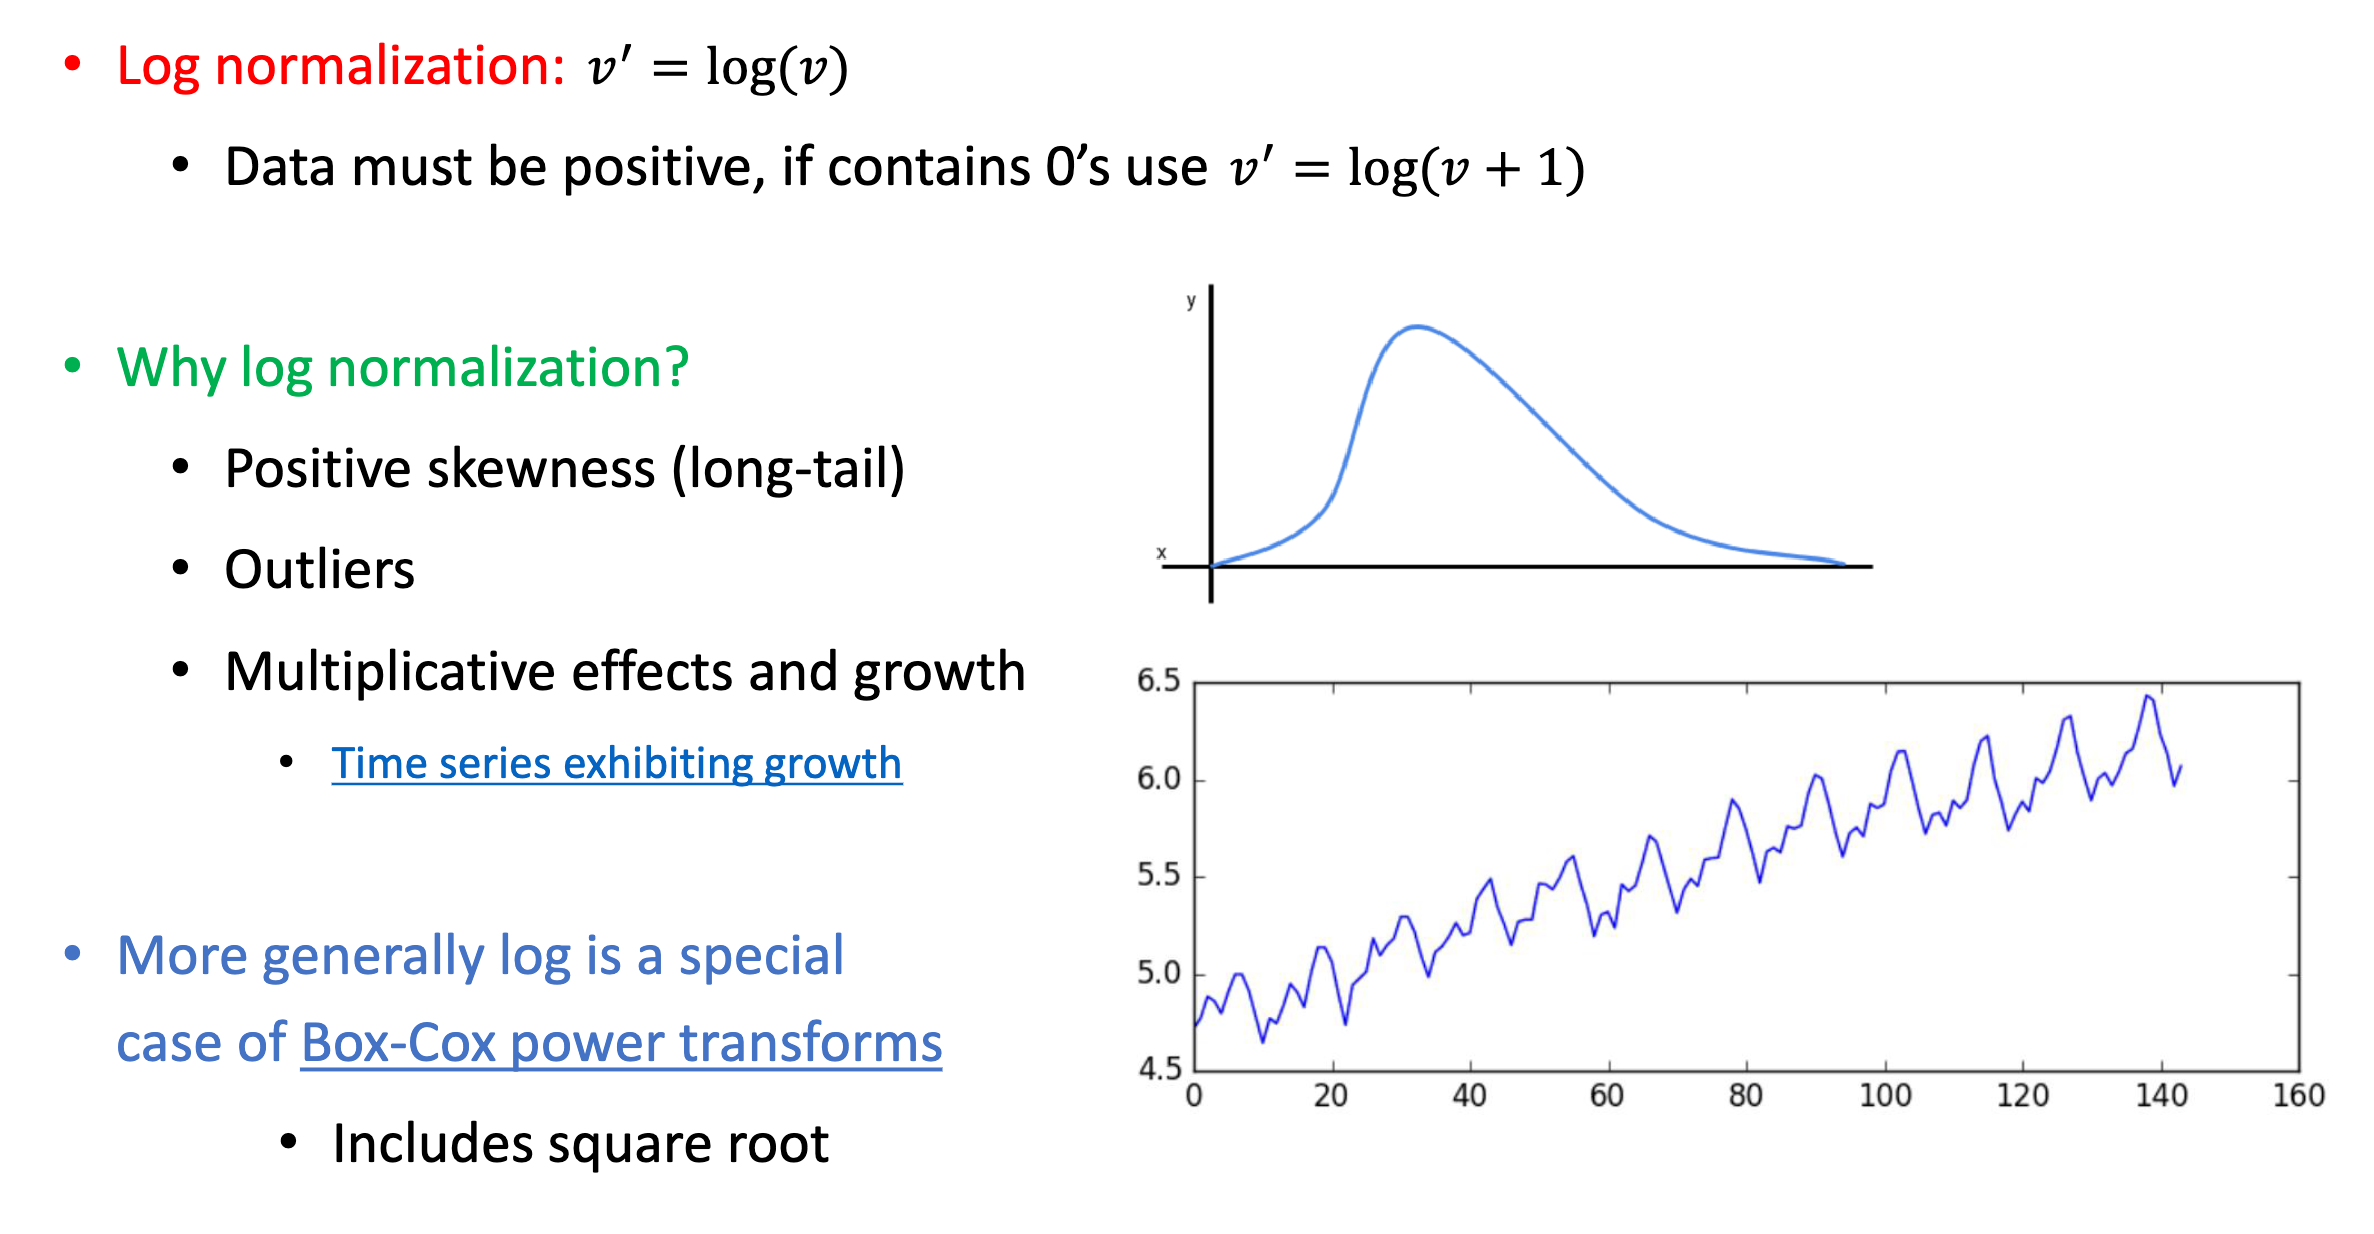
\includegraphics[width=\textwidth/2]{19.png}
\end{document}